% Header mit Deklarationen
\documentclass[%
	%pdftex,%              PDFTex verwenden
	a4paper,%             A4 Papier
	oneside,%             Einseitig
	bibtotoc,%    		Literaturverzeichnis einf�gen bibtotocnumbered: nummeriert
	liststotoc,%		Verzeichnisse einbinden in toc
	idxtotoc,%            Index ins Verzeichnis einf�gen
	halfparskip,%        Europ�ischer Satz mit abstand zwischen Abs�tzen
	chapterprefix,%       Kapitel anschreiben als Kapitel
	headsepline,%         Linie nach Kopfzeile
	%footsepline,%         Linie vor Fusszeile
	%pointlessnumbers,%     Nummern ohne abschlie�enden Punkt
	12pt%                 Gr�ssere Schrift, besser lesbar am bildschrim
]{scrbook}

%
% Paket f�r �bersetzungen ins Deutsche
%
\usepackage[french,ngerman]{babel}

%
% Pakete um Latin1 Zeichnens�tze verwenden zu k�nnen und die dazu
% passenden Schriften.
%
\usepackage[latin1]{inputenc}
\usepackage[T1]{fontenc}

%
% Paket f�r Quotes
%
\usepackage[babel,french=guillemets,german=swiss]{csquotes}

%
% Paket zum Erweitern der Tabelleneigenschaften
%
\usepackage{array}

%
% Paket f�r sch�nere Tabellen
%
\usepackage{booktabs}

%
% Paket um Grafiken einbetten zu k�nnen
%
\usepackage{graphicx}

%
% Spezielle Schrift im Koma-Script setzen.
%
\setkomafont{sectioning}{\normalfont\bfseries}
\setkomafont{captionlabel}{\normalfont\bfseries} 
\setkomafont{pagehead}{\normalfont\bfseries} % Kopfzeilenschrift
\setkomafont{descriptionlabel}{\normalfont\bfseries}

%
% Zeilenumbruch bei Bildbeschreibungen.
%
\setcapindent{1em}

%
% Kopf und Fu�zeilen
%
\usepackage{scrpage2}
\pagestyle{scrheadings}
% Inhalt bis Section rechts und Chapter links
\automark[section]{chapter}
% Mitte: leer
\chead{}

%
% mathematische symbole aus dem AMS Paket.
%
\usepackage{amsmath}
\usepackage{amssymb}

%
% Type 1 Fonts f�r bessere darstellung in PDF verwenden.
%
%\usepackage{mathptmx}           % Times + passende Mathefonts
%\usepackage[scaled=.92]{helvet} % skalierte Helvetica als \sfdefault
\usepackage{courier}            % Courier als \ttdefault

%
% Paket um Textteile drehen zu k�nnen
%
\usepackage{rotating}

%
% Paket f�r Farben im PDF
%
\usepackage{color}

%
% Paket f�r Links innerhalb des PDF Dokuments
%
\definecolor{LinkColor}{rgb}{0,0,0.5}
\usepackage[%
	pdftitle={Nachrichtenaustausch unter Angriff},% Titel der Diplomarbeit
	pdfauthor={Thomas Bosch},% Autor(en)
	pdfcreator={LaTeX, LaTeX with hyperref and KOMA-Script},% Genutzte Programme
	pdfsubject={Diplomarbeit}, % Betreff
	pdfkeywords={Nachrichten, Angriff, DDoS, Bedrohungen, Kritische Infrastrukturen}]{hyperref} % Keywords halt :-)
\hypersetup{colorlinks=true,% Definition der Links im PDF File
	linkcolor=LinkColor,%
	citecolor=LinkColor,%
	filecolor=LinkColor,%
	menucolor=LinkColor,%
	pagecolor=LinkColor,%
	urlcolor=LinkColor}

%
% Paket um LIstings sauber zu formatieren.
%
\usepackage[savemem]{listings}
\lstloadlanguages{TeX}

%
% Listing Definationen f�r PHP Code
%
\definecolor{lbcolor}{rgb}{0.85,0.85,0.85}
\lstset{language=[LaTeX]TeX,
	numbers=left,
	stepnumber=1,
	numbersep=5pt,
	numberstyle=\tiny,
	breaklines=true,
	breakautoindent=true,
	postbreak=\space,
	tabsize=2,
	basicstyle=\ttfamily\footnotesize,
	showspaces=false,
	showstringspaces=false,
	extendedchars=true,
	backgroundcolor=\color{lbcolor}}
%
% ---------------------------------------------------------------------------
%

%
% Neue Umgebungen
%
\newenvironment{ListChanges}%
	{\begin{list}{$\diamondsuit$}{}}%
	{\end{list}}

%
% aller Bilder werden im Unterverzeichnis figures gesucht:
%
\graphicspath{{bilder/}}

%
% Literaturverzeichnis-Stil
%
\bibliographystyle{plain}

%
% Strukturiertiefe bis subsubsection{} m�glich
%
\setcounter{secnumdepth}{3}
\setcounter{tocdepth}{3}

% 
% Hurenkinder und Schusterjungen
%
\clubpenalty = 10000
\widowpenalty = 10000
\displaywidowpenalty = 10000


\begin{document}

% R�mische Nummerierung f�r Sonderseiten, wie Verzeichnisse und Anhang
\pagenumbering{Roman}

% Titelblatt
% Die Titelseite
% Im folgenden kommen ein paar Variablen, die auszuf�llen sind
% Bisher steht dort nur Musterinhalt
% Au�erdem m�ssen zei Dateien erstellt werden, Bild/Logo/Emblem des Fachgebietes
% sowie der Universit�t

\newcommand{\trtitle}{Nachrichtenaustausch unter Angriff}
\newcommand{\trtype}{Diplomarbeit}
\newcommand{\trauthor}{Thomas Bosch}
\newcommand{\trstrasse}{Warschauer Str. 82}
\newcommand{\trmatrikelnummer}{197609}
\newcommand{\trort}{10243 Berlin}
\newcommand{\trbetreuerA}{Dipl.-Inform. Olaf Kroll-Peters}
\newcommand{\trbetreuerB}{Dipl.-Inform. Rainer Bye}
\newcommand{\trprof}{Prof.\ Dr.-Ing.\ habil.\ Sahin Albayrak}
\newcommand{\trfachgebiet}{Agententechnologien in betrieblichen Anwendungen und der Telekommunikation}
\newcommand{\trinstitut}{Wirtschaftsinformatik und Quantitative Methoden}
\newcommand{\trfakultaet}{IV Elektrotechnik und Informatik}
\newcommand{\truni}{Technische Universit�t Berlin}
\newcommand{\trdate}{\today}

\thispagestyle{empty}

% Kopfzeile mit Logos.
% Eventuell die \hspace{} je nach Logogr��e anpassen
\begin{tabular}{lcr}
  
\includegraphics[scale=0.4]{tu_logo_rot} & % dein_unilogo.jpg/.eps im Verzeichnis "bilder" ablegen
  \hspace{3cm} \truni \hspace{2cm} &
  
\includegraphics[scale=0.5]{dailogo} % dein_fglogo.jpg/.eps im Verzeichnis "bilder" ablegen, Fachgebietslogo
  \\
\end{tabular}

\rule{\textwidth}{0.4pt}

\vspace{2.5cm}
\begin{center}
  \textbf{\LARGE \trtitle}
\end{center}
\vspace{2cm}

\begin{center}
  \textbf{\trtype} \\
  am Fachgebiet \trfachgebiet \\
  \trprof \\
  Institut f�r \trinstitut \\
  Fakult�t \trfakultaet \\
  \truni \\[0.5cm]
  vorgelegt von \\
  \textbf{\trauthor}
\end{center}

\vspace{1cm}


\begin{center}
\begin{tabular}{ll}
Betreuer: & \trbetreuerA \\
 					& \trbetreuerB
\end{tabular}
\end{center}

\vfill

\begin{tabular}{l}
\trauthor \\
Matrikelnummer:  \trmatrikelnummer \\
\trstrasse \\
\trort
\end{tabular}

\rule{\textwidth}{0.4pt}


% Verzeichnisse
% Kopfzeile links Kapitel, rechts leer
\ihead{\leftmark}
\ohead{}
\tableofcontents

\listoffigures

\listoftables


% Merke mir die r�mische Seitenzahl in 'roemisch' und setzte Nummeriernung 
% auf arabisch f�r die eigentlichen Kapitel
\newpage
\newcounter{roemisch}
\setcounter{roemisch}{\value{page}}
\pagenumbering{arabic}

% Die einzelnen Kapitel
% Kopfzeile: links Kapitel, rechts Sektion
\ihead{\leftmark}
\ohead{\rightmark}
\chapter{Einleitung}
\label{cha:einleitung}
In den vergangenen Jahrzehnten hat das Thema Netzwerksicherheit (Network Security) immer mehr an Bedeutung gewonnen. Mit wachsenden IT-Strukturen wachsen auch die M�glichkeiten diese Strukturen anzugreifen. In den kommenden Jahren wird die Sicherheit in Netzwerken immer mehr zu einem zentralen Forschungsthema werden.

\section{Motivation}
Ausgehend von den stetig wachsenden IT-Strukturen gibt es immer mehr Menschen, die diese auch nutzen. Diese Entwicklung wird folgend mit statistischen Erhebungen belegt. Es wird gezeigt, wie sich dieser Wachstum auswirkt und welche M�glichkeiten dadurch f�r potentielle Angreifer geschaffen werden.  

\subsection{Was ist}
Die Zahl der Internetnutzer in Deutschland ist, wie in Abbildung~\ref{fig:internetnutzer} zu sehen, in den vergangenen Jahren von 1997 bis 2004 von $4,1$ auf $35,7$ Millionen gestiegen. Allein in diesen sieben Jahren hat sich die Nutzerzahl fast verneunfacht.
\begin{figure}[htb]
\centering
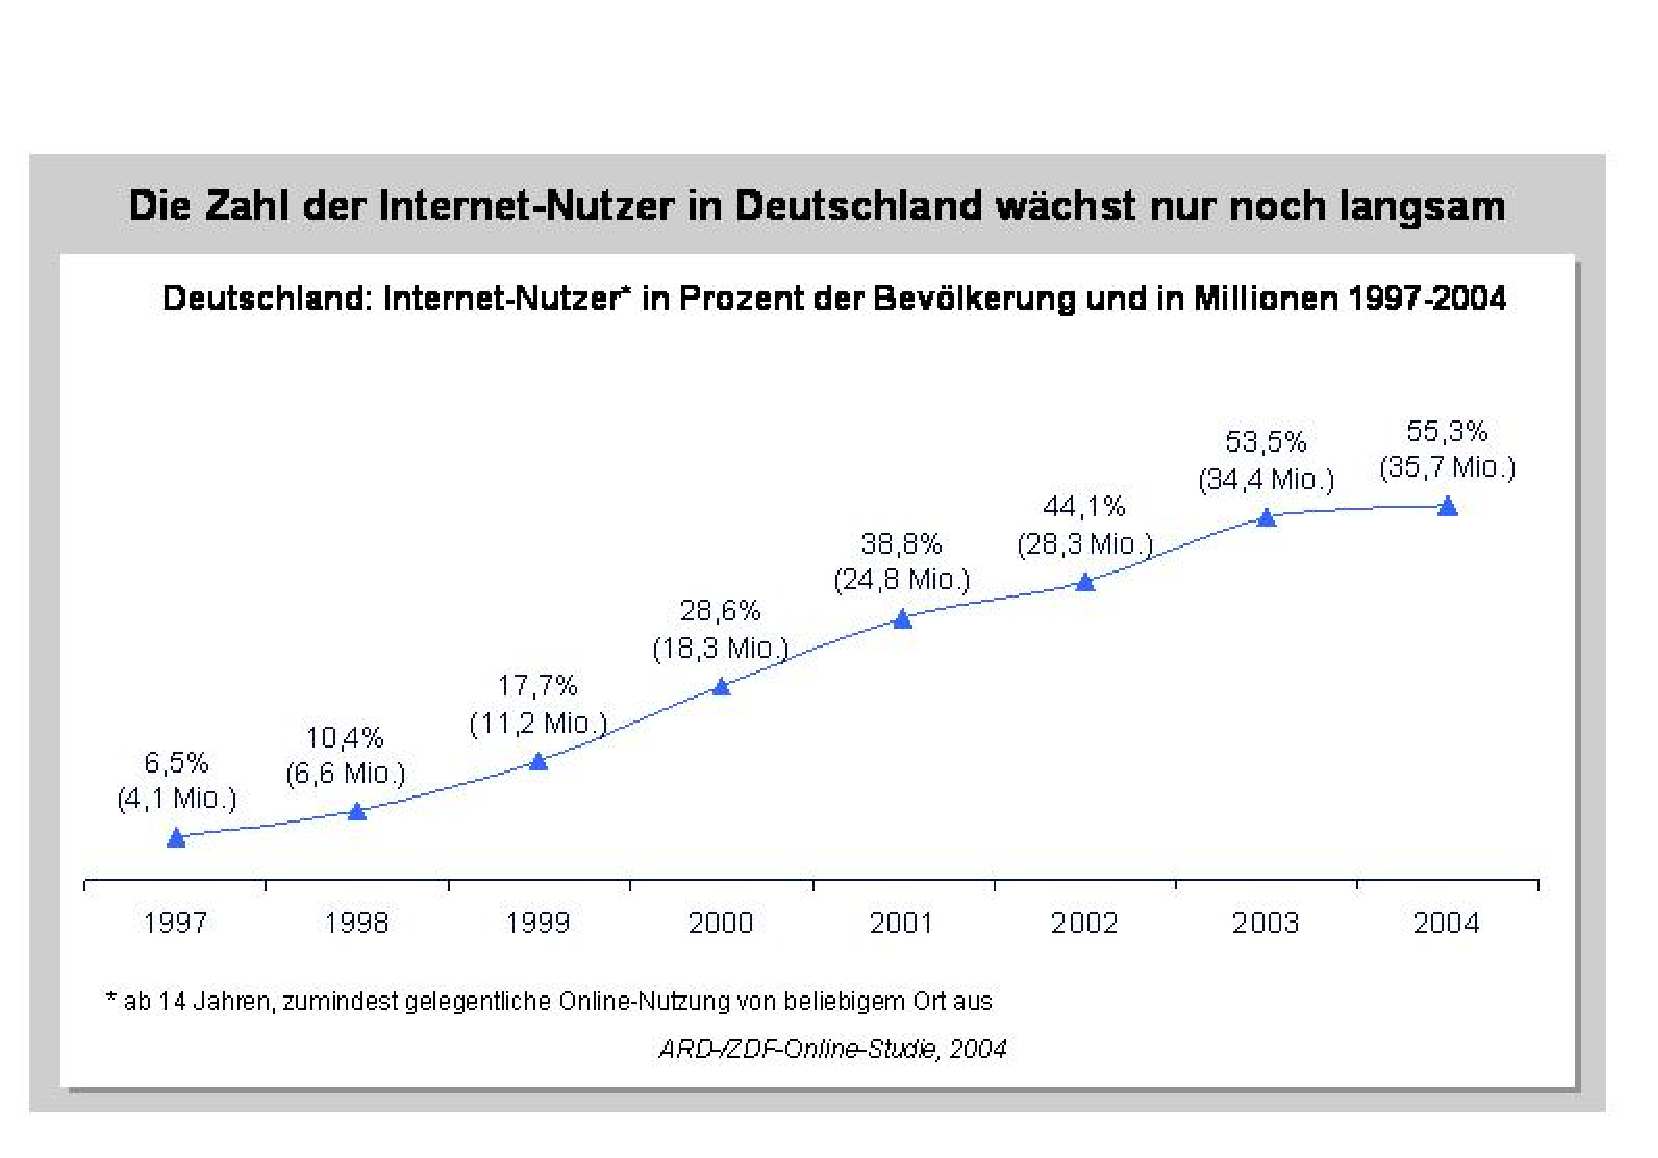
\includegraphics[width=0.7\textwidth]{folie215}
\caption{Anzahl der Internetnutzer in Deutschland - Quelle: Infratest\cite{infratest215}} 
\label{fig:internetnutzer}
\end{figure}
Somit stiegen auch die M�glichkeiten Angriffe auf Computernetzwerke auszuf�hren. Mit steigender Anzahl an Nutzern werden auch mehr Ressourcen ben�tigt, um diese Flut an Daten bew�ltigen zu k�nnen. Das sog. \textit{Backbone} des Internets, d.h. die Verbindung von Routern und Gateways �ber die der gesamte Verkehr flie�t, musste demnach ebenfalls ausgebaut werden. Mehr Rechner bedeuten dann wieder mehr Angriffspunkte f�r potentielle Angreifer.

Bis 2008 werden es laut Infratest\cite{infratest217} sogar $75,6$ Millionen Menschen in Deutschland sein, die das Internet nutzen. Hierbei ist zu beachten, dass verschiedene Institute auch verschiedene Herangehensweisen zur Erhebung der Sch�tzungen haben und je nach Definition des Begriffs "`Nutzung"' auch verschiedene Werte entstehen. So definiert das Institut EITO (European Information Technology Observatory) den Begriff Nutzer als: "`Personen, die das Internet mindestens einmal im Monat nutzen, unabh�ngig vom Alter  und Nutzungsort"'\cite{infratest217}. In Abbildung~\ref{fig:institute} ist zu sehen, dass die Zahlen unterschiedlich sind, abh�ngig vom Institut.
\begin{figure}[htb]
\centering
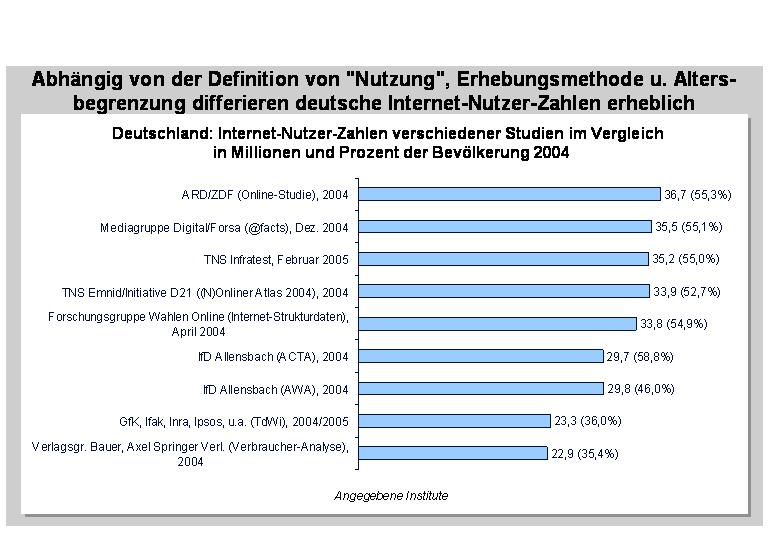
\includegraphics[width=0.7\textwidth]{folie216}
\caption{Verschiedene Institute im Vergleich - Quelle: Infratest\cite{infratest216}}
\label{fig:institute}
\end{figure}

Wie in Abbildung~\ref{fig:international} zu sehen ist, sehen die weltweiten Sch�tzungen im Vergleich zu den Sch�tzungen, die die deutsche Bev�lkerung wiedergeben, nicht anders aus. Dort ist ein Wachstum des Internets von 1999 bis 2008 von $286$ Millionen auf $1,28$ Milliarden Nutzer zu sehen, was innerhalb von 4 Jahren eine Verdopplung bedeutet.
\begin{figure}[htb]
\centering
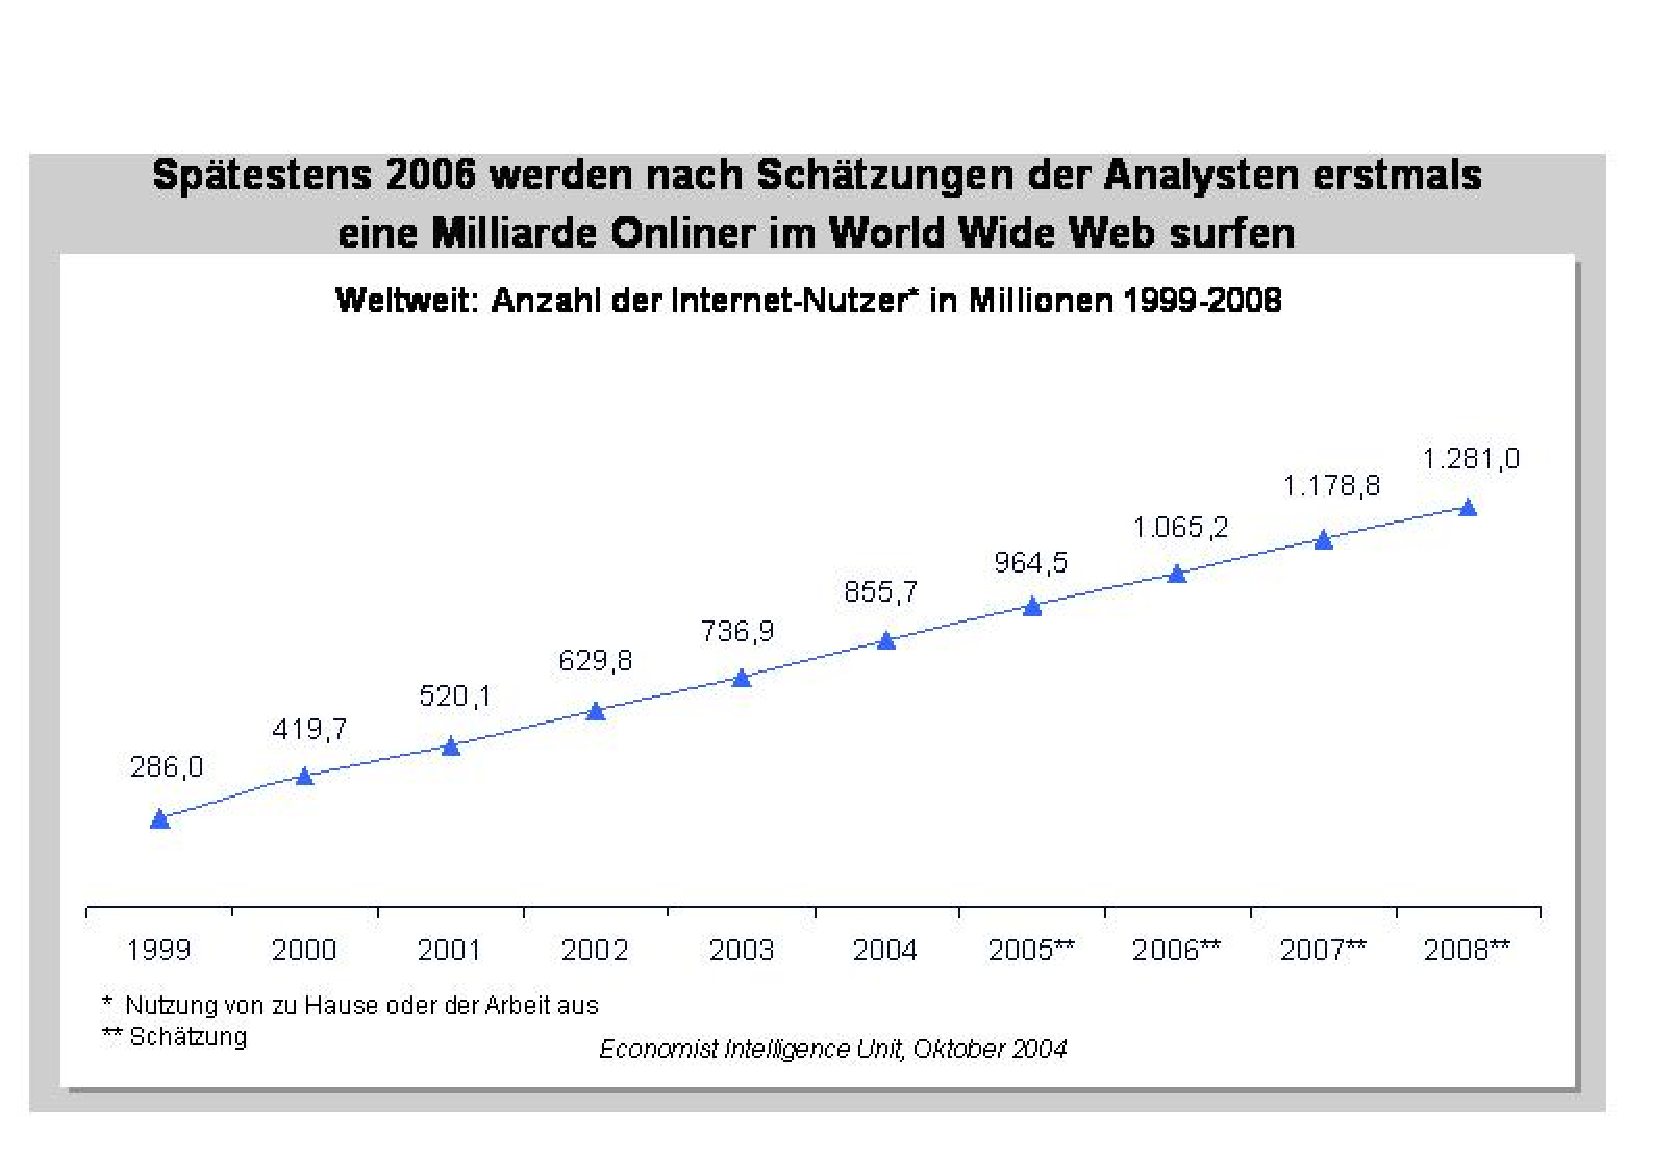
\includegraphics[width=0.7\textwidth]{folie186}
\caption{Internationales Internetwachstum - Quelle: Infratest\cite{infratest186}} 
\label{fig:international}
\end{figure}

Neben den privaten Nutzern sind es aber auch vor allem gewerbliche und staatliche Einrichtungen, die immer vermehrter die Ressourcen des Internets nutzen. So gibt es beispielsweise Internetplatformen der \textit{Agentur f�r Arbeit}\footnote{\url{http://www.agenturfuerarbeit.de}} oder gewerbliche Nutzung, wie die Handelsplatform \textit{ebay}\footnote{\url{http://www.ebay.de}}. Viele Arbeitspl�tze und ein stetig steigender Anteil am Bruttoinlandsprodukt sind direkt oder indirekt mit dem Internet verkn�pft. Die gesamtwirtschaftliche Bedeutung der IKT (Informations- und  Kommunikationstechnologien) hat sich von $4,7\%$ im Jahr 1995 auf $6,8\%$ im Jahr 2004 erh�ht\cite{statistischesbundesamt}. Der genannte Prozentsatz bezieht sich auf den Anteil der IKT-Waren und IKT-Dienstleistungen am deutschen Bruttoinlandsprodukt. Dies ist nur die gewerbliche Form der Nutzung von IT-Strukturen. Weitere �ffentliche Einrichtungen werden ebenso immer abh�ngiger von den Ressourcen des Internets.

Weiterhin gibt es Strukturen, auch \textit{Kritische Infrastrukturen} genannt, die f�r die deutsche Gesellschaft von sehr gro�er Bedeutung sind.
\begin{quotation}
Organisationen und Einrichtungen mit wichtiger
Bedeutung f�r das staatliche Gemeinwesen, bei
deren Ausfall oder Beeintr�chtigung nachhaltig
wirkende Versorgungsengp�sse, erhebliche
St�rungen der �ffentlichen Sicherheit oder andere
dramatische Folgen eintreten w�rden.
\begin{flushright}
(2004)
\end{flushright}
\end{quotation}

Hierbei handelt es sich um ein Zitat\cite{kritis} des BSI (Bundesministerium f�r Sicherheit in der Informationstechnik). Kritische Infrastrukturen sind in Deutschland beispielsweise Transport und Verkehr, Energie, Finanzwesen, Versorgung oder Justiz. Alle diese Sektoren haben in Deutschland eine wichtige Bedeutung und deren Beeintr�chtigung w�re f�r die Gesellschaft schwer zu verkraften. Durch verschiedenartige Angriffe k�nnten solche Beeintr�chtigungen stattfinden. 

\subsection{Was sein k�nnte}
Fehlerhafte Software, Schadprogramme (z.B. Trojaner), Angriffe von innen und au�en aber auch physische Einwirkungen, wie Blitzeinschl�ge oder terroristische Anschl�ge k�nnen die Funktionalit�t von Netzwerken behindern. Da Kritische Infrastrukturen kommunizieren auch �ber Netzwerke. Sie bilden ein Intranet. So k�nnen beispielsweise verschiedene Kontrollsysteme innerhalb dieses Intranets von beliebiger Stelle abgefragt werden k�nnen. Diese internen Netzwerke sind auch, genau wie das Internet durch unterschiedliche Faktoren bedroht. So k�nnen auch hier fehlerhafte Software oder Trojaner den Nachrichtenaustausch beeintr�chtigen. Die Beeintr�chtigung eines der Sektoren von Kritischen Infrastrukturen, z.B. des Transportsektors h�tte alleine f�r den Wirtschaftsstandort Deutschland verheerende Folgen.

Ein gezielter Angriff auf das Verkehrsleitsystem der Deutschen Bahn k�nnte den Ausfall von lokalen Betriebsstrecken bedeuten. M�glicherweise k�nnte es sogar zu einem bundesweiten Ausfall kommen. Dieses Beispiel zeigt, wie relevant die Sicherung solcher Strukturen ist. Es muss jederzeit gew�hrleistet sein, dass der Nachrichtenaustausch innerhalb der Netzwerke funktioniert. Daher sind Sicherstellungen der Verf�gbarkeit, Integrit�t und Vertraulichkeit der Kritischen Infrastrukturen Hauptschutzziel des BSI.

Mit steigender Nutzung der von Netzwerktechnologie in der Gesellschaft steigt auch die Gefahr, dass diese Technologie
angegriffen wird. Der Nachrichtenaustausch in Netzwerken muss auch f�r den Fall garantiert sein, dass dieses Netzwerk angegriffen wird. Um das Verhalten eines Netzwerks oder einzelner Netzwerkkomponenten zu untersuchen, werden Netzwerksimulatoren entwickelt. Diese Simulatoren k�nnen der �berpr�fung und Bewertung neu entwickelter Verteidigungsstrategien dienen.

\section{Ziel der Arbeit}
Diese Arbeit behandelt unterschiedliche Bedrohungen der Verf�gbarkeit, Integrit�t und Vertraulichkeit von Netzwerken. Zu Beginn wird dies in einer theoretischen Betrachtung vertieft. Dieser theoretische Hintergrund dient dann dazu, nachzuvollziehen, wie sich solche in der Theorie bekannten Bedrohungen in der Praxis auswirken. Solche Bedrohungen beeintr�chtigen den Nachrichtenaustausch innerhalb von Netzwerken. 

Ziel ist es, die Bedeutsamkeit des Nachrichtenaustauschs innerhalb von Netzwerken darzustellen. Weiterhin soll in einer Simulation die Bedrohung und der Angriff eines Netzwerks implementiert und auf diesen reagiert werden. Dazu wird eine Gegenma�nahme integriert, die dann den Austausch von Nachrichten w�hrend eines stattfindenen Angriffs weiterhin erm�glicht.

\section{Aufbau der Arbeit}
Um dieses Ziel zu erreichen, wird in Kapitel~\ref{cha:sota} zun�chst der aktuelle Stand der Wissenschaft geschildert.

In Kapitel~\ref{cha:theorie} werden dann ein paar Grundlagen im Thema Netzwerke erl�utert anhand derer dann Bedrohungen und Sch�den durch Angriffe auf IT-Strukturen betrachtet werden. Weiterhin wird dort untersucht, inwieweit solche Angriffe zu verhindern sind. Welche Gegenma�nahmen existieren, um einen Angriff zumindest einzud�mmen?

Zudem gibt es in Kapitel~\ref{cha:theorie} noch einen historischen R�ckblick, bei dem auf schon stattgefundene Angriffe eingegangen wird. Diese werden erl�utert und es wird aufgezeigt, welche Ma�nahmen bisher gegen die Verteidigung solcher Angriffe ergriffen wurden. Was lassen sich au�erdem aus diesen Angriffen f�r Erkenntnisse mitnehmen? Wurde aus den Erfahrungen gelernt? F�r den Fall, dass alle Ma�nahmen der Abwehr scheitern, bleibt zuletzt nur noch die M�glichkeit andere Wege f�r den Nachrichtenaustausch zu finden. Wie k�nnen solche Notfallpl�ne aussehen? Welche anderen Ressourcen lassen sich hierzu nutzen? Es werden einige alternative Wege des Nachrichtenaustauschs heraus gestellt, wobei positive und negative Eigenschaften dieser Alternativen aufgezeigt werden.

Kapitel~\ref{cha:praxis} beschreibt die Herangehensweise und Implementierung eines ausgew�hlten Angriffs in einem, im DAI-Labor entwickelten Netzwerksimulator namens \textbf{NeSSi} (Network Security Simulator). Weiterhin wird die Simulation eines Angriffs dann bewertet. Was passiert nun wirklich w�ren des Angriffs? Was bewirken die Gegenma�nahmen, die nach dem Angriff eingeleitet werden, oder schon pr�ventiv eingeleitet wurden? Dieser praktische Teil soll den theoretischen Teil unterst�tzen und die darin enthaltenen Ans�tze zur L�sung des Problems "`Nachrichtenaustausch unter Angriff"' untersuchen.

Zuletzt wird in Kapitel~\ref{cha:fazit} ein Fazit gezogen. Was l�sst sich den Ergebnissen der Simulation entnehmen? Hier werden die Ergebnisse abschlie�end bewertet und in einen Ausblick integriert.

Bevor theoretische und praktische Aspekte in den Vordergrund treten, wird  im folgenden Kapitel zun�chst auf den aktuellen Stand der Wissenschaft eingegangen und deren Erkenntnisse zu diesem Thema dargelegt.

\chapter{State of the Art}
\label{cha:sota}
In den letzten Jahren wurde das Thema \textit{Angriffe auf Netzwerke und deren Bek�mpfung} immer intensiver in der Wissenschaft erforscht. Bereits im Jahr 1990 wurde von Heady et al.\cite{heady} die Erkennung von Anomalien in Netzwerken behandelt. So wurden in den folgenden Jahren viele Systeme entwickelt, die sich mit dieser Anomalieerkennung besch�ftigen, wie beispielsweise die LOF-Methode (\textit{Local Outlier Factor}) von Breuning et al.\cite{lof}. Aber auch andere Methoden wurden entwickelt. Damit stieg die Notwendigkeit des Vergleiches, so dass von Lazarevic et al.\cite{lazarevic} verschiedene Methoden zur Anaomalieerkennung getestet und miteinander verglichen werden. Die erw�hnte LOF-Methode wird dabei als die zuverl�ssigste bewertet.

Neben der Anomalieerkennung sind weitere Methoden zum Schutz von Netzwerken entworfen worden. Verschiedenste Filter wurden entwickelt um \textit{Distrisbuted Denial-of-Service} (DDoS: siehe Abschnitt~\ref{sec:ddos}) einzud�mmen. So haben Keromytis et al.\cite{sos} eine Methodik zur Verminderung von DoS entwickelt, welche nur authentifizierten Paketen erlaubt ein bestimmtes Ziel zu erreichen. So ein Overlay-basiertes Filtern wurde auch von Weiteren\cite{doslimiting,mayday} untersucht. Weiterhin wurden Filtermethoden vorgeschlagen, die das \textit{Spoofen} von IP-Adressen verhindern sollen\cite{filtersource} oder durch sogenanntes \textit{traceback}, d.h. durch eine schrittweise R�ckverfolgung, die Quellen solcher Attacken herausfiltern\cite{iptraceback,iptraceback2}. Eine dritte Methode, das \textit{pushback}\cite{pushback,pushback2}, erm�glicht das Platzieren von Netzwerkfiltern in Netzwerken, die der Quelle der Attacke n�her sind.

Im Bereich der Verhinderung bzw. Abschw�chung von Angriffen auf gro�e Netzwerke wurde schon viel geforscht. Die Forschung ist bisher jedoch noch auf der Suche nach dem Optimum. Bisher wurde noch keine Methode gefunden beispielsweise DDoS wirksam zu bek�mpfen.

Die Entwicklung von Gegenma�nahmen gegen Angriffe auf Netzwerke bzw. einzelne Teilnehmer von Netzwerken ben�tigt zun�chst theoretische Kenntnisse. Dazu geh�ren Wissen �ber Aufbau von Netzwerken. Zudem auch die Kenntnisse �ber die Methoden von Angriffen. Diese Theorie wird im folgenden Kapitel er�rtert.

\chapter{Theoretischer Hintergrund}
\label{cha:theorie}
In diesem Kapitel wird der Hintergrund eines \textit{Nachrichtenaustauschs unter Angriff} theoretisch erl�utert. Dazu werden zun�chst Grundlagen geschaffen, auf denen dann in den weiteren Kapitel aufgebaut wird. So werden Bedrohungen von Netzwerken genannt und in einem historischen R�ckblick exemplarisch dargelegt. Mit diesen Kenntnissen und Grundlagen lassen sich dann m�gliche Verteidigungstrategien entwickeln.

\section{Grundlagen}
Zuerst einmal wird der Begriff "`Netzwerk"' etwas n�her gebracht. Ein Netzwerk beschreibt im allgemeinen eine Verkn�pfung mehrerer Computer untereinander, so dass diese miteinander kommunizieren k�nnen. Das Internet ist das gr��te Netzwerk das wir kennen. Es beschreibt die Verkn�pfung tausender Netzwerke weltweit.

Um nun miteinander kommunizieren zu k�nnen und die Komplexit�t einer solchen Kommunikation von Millionen von Computern im Rahmen zu halten, bedarf es einer Verteilung verschiedener Aufgaben auf einzelne Teilbereiche, \textbf{Layer} genannt. Ich benutzte im weiteren Verlauf die deutsche �bersetzung, Ebene.

Jede Ebene ist nun eine Ansammlung von Protokollen, die nun bestimmte Funktionalit�ten bieten. So �bernimmt eine Ebene beispielsweise die physikalische �bertragung, eine andere gew�hrleistet das Finden des Empf�ngers und eine weitere sorgt f�r die verlustfreie �bertragung.

\subsection{Das ISO/OSI-Modell}
Ein Modell, welches nun die Aufgaben einer jeden Ebene definiert, ist das \textbf{ISO/OSI-Referenzmodell}. Es wurde 1983 als ISO-Standard (International Standards Organization) eingetragen\cite{tanenbaum}. Das ISO/OSI-Modell definiert sieben Ebenen, wie sie in Abbildung~\ref{fig:isoosi} zu sehen sind. Die Ebenen wurden so geschaffen, dass folgende Punkte gew�hrleistet sind\cite{tanenbaum}:
\begin{itemize}
% \labelitemi -
 \item Jede Ebene sollte ein eigene Abstraktionsebene bilden
 \item Jede Ebene sollte eine wohl definierte Aufgabe haben
 \item Die Aufgabe jeder Ebene sollte sich nach den internationalen Protokollstandards richten
 \item Der Datenfluss zwischen den Ebenen sollte m�glichst gering gehalten werden
 \item Die Anzahl der Ebenen sollte so gew�hlt sein, dass Aufgaben sich nicht �berschneiden, aber die �bersichtlichkeit gewahrt wird 
\end{itemize}

\begin{figure}[htb]
 \centering
 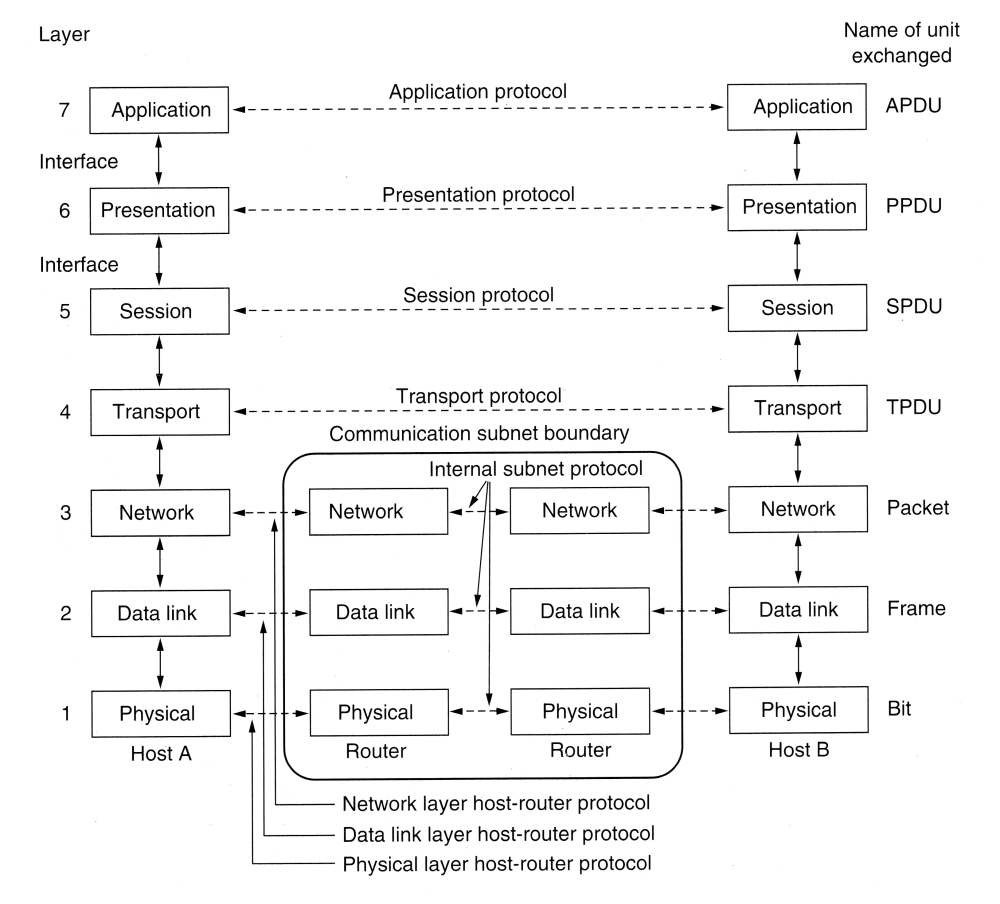
\includegraphics[width=0.8\textwidth]{isoosi}
 \caption{Das ISO/OSI-Ebenenmodell - Quelle: Tanenbaum\cite{tanenbaum}}
 \label{fig:isoosi}
\end{figure}

\subsection{TCP/IP-Modell}
Neben dem ISO/OSI-Modell wurde 1974 auch das \textbf{TCP/IP-Referenzmodell} definiert\cite{cerfkahn}. In diesem Modell gibt es nur vier Ebenen. Verglichen mit dem ISO/OSI-Modell wurden beim TCP/IP-Modell die ersten beiden Ebenen, deren Aufgaben eher physikalischer Natur sind, zusammengelegt. Wie in Abbildung~\ref{fig:tcpip} erkennbar ist, wurden weiterhin die Ebenen f�nf und sechs komplett ausgespart.
\begin{figure}[htb]
 \centering
 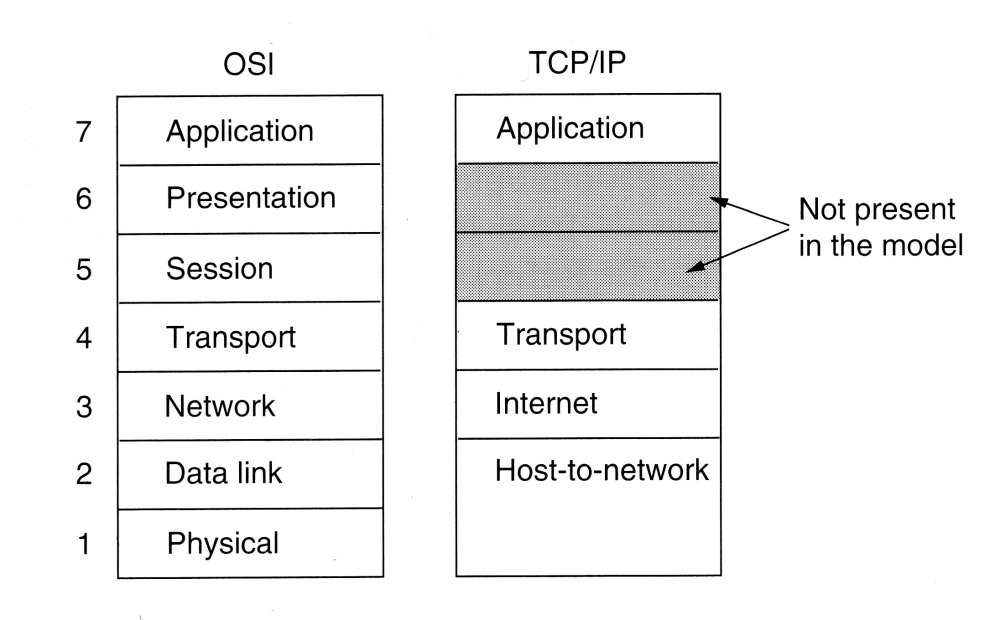
\includegraphics[width=0.8\textwidth]{tcpip}
 \caption{Das TCP/IP-Ebenenmodell im Vergleich - Quelle: Tanenbaum\cite{tanenbaum}}
 \label{fig:tcpip}
\end{figure}

Der weiter Verlauf der Arbeit wird sich nur mit den Ebenen \textit{Applikation}, \textit{Transport}, \textit{Internet} bzw. \textit{Netzwerk} und \textit{Physikalisch} bzw. \textit{Host-to-Network} besch�ftigen. Im Folgenden werden nun diese vier Ebenen n�her erl�utert und ein paar Beispiele verdeutlichen die Funktionsweise der einzelnen Ebenen.

\subsection{Host-to-Network Ebene}
Die Host-to-Network Ebene bildet die Basis der Daten�bertragung. Sie handhabt die physikalische �bertragungsweise. Eine Art w�re die �bertragung �ber Lichtwellenleiter, eine andere die elektrische �bertragung �ber die �blichen Kupferkabel. Neben dieser untersten Basisfunktionalit�t bietet sie aber auch noch die Funktionalit�t der im ISO/OSI-Modells Data-Link-Layer genannten Ebene. Diese bietet Funktionen, wie die Behandlung von Fehlern. Fehler k�nnen etwa durch physikalische Einfl�sse, wie Leitungsrauschen entstehen.

\subsection{Netzwerkebene}
Diese Ebene ist f�r den korrekten Versand von einzelnen Paketen durch ein Netzwerk verantwortlich. Das zugrunde liegende Protokoll ist das \textbf{IP-Protokoll}. Mit Hilfe dieses Protokolls und verschiedener Routingalgorithmen wird auf der Netzwerkebene sichergestellt, dass jedes erhaltene Paket korrekt weitergeleitet wird. 

\subsubsection{IP-Protokoll}
Das IP-Protokoll wird auch umgangssprachlich das "`Internet-Protokoll"' genannt. Es ist das Protokoll auf das alle anderen Protokolle, wie TCP, UDP oder ICMP aufsetzen. Es beinhaltet keine Verbindungsmethoden, jedoch eine Paket-Struktur.
\begin{figure}[htb]
\centering
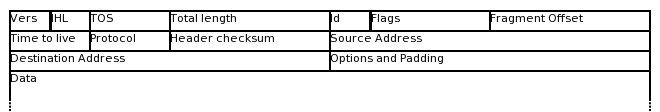
\includegraphics[width=0.8\textwidth]{ip}
\caption{Aufbau eines IP-Pakets}
\label{fig:ippaket}
\end{figure}

Jeder Computer im Internet hat eine Adresse mit der er eindeutig verkn�pft ist, die \textit{IP-Adresse}. Diese IP-Adresse ist ein 4 Byte langes Feld, das zur besseren Lesbarkeit in vier, durch Punkte getrennte Dezimalzahlen von 0 bis 255 notiert wird. Also beispielsweise 243.155.5.56. Anhand dieser Adressierung ist es somit m�glich, dass ein Nachrichtenaustausch, also die Kommunikation, von einer Seite der Erde auf die andere ohne gro�e M�he funktioniert. Dieser Nachrichtenaustausch erfolgt �ber Nachrichtenpakete, die verschiedenste Informationen, wie Absender, Empf�nger und nat�rlich auch Daten enthalten.

Wie in Abbildung~\ref{fig:ippaket} zu sehen ist, beinhaltet ein solches IP-Paket noch viel mehr Informationen auf die hier aber nicht eingegangen wird. Wichtig sind erst einmal nur die Adressen, also \textit{Destination Address} und \textit{Source Address}.

\subsubsection{Routing-Protokolle}
Die Routing-Protokolle erm�glichen den dynamischen Aufbau von Routing-Tabellen in jedem einzelnen Router (siehe Abschnitt~\ref{sec:router}). Die von den Protokollen genutzten Algorithmen lassen sich in zwei Klassen aufteilen.
\begin{description}
\item[Link-State-Protokoll] Bei diesem Algorithmus wird allen anderen Routern mitgeteilt, welche Nachbarn jeder einzelne Router hat. Somit kann jeder Router f�r sich aus den Informationen der anderen eine Topologie aufbauen und seine Routingtabelle danach erstellen.
\item[Distance-Vector-Protokoll] Hier teilt jeder Router seinen Nachbarn mit, welche Router ihm bekannt sind und mit wie vielen Schritten diese erreicht werden k�nnen. Unter diese Art von Protokollen fallen auch die mit einem verbesserten Algorithmus versehenen Pfadvektor-Protokolle, wie das \textit{BGP} (Border Gateway Protocol).
\end{description}
In diese Klassen fallen nun verschiedene Protokolle, die die Router nutzen, um ihre Pakete m�glichst schnell an sein Ziel zu weiterzuleiten.

\subsubsection{ICMP}
Dieses Protokoll wird f�r Kontrollzwecke genutzt. ICMP (\textit{Internet Control Management Protocol}) bietet Funktionalit�ten, die f�r das Management von Verbindungen im Netzwerk n�tig sind. So sendet ein Router dem Sender eines Paketes ein ICMP-Paket vom Typ "`Destination Unreachable"' und dem Code "`Host Unreachable"'\cite{rfc792icmp}, wenn der Empf�nger, welcher im Header des IP-Paketes enthalten ist nicht in seinem Netzwerk existiert.

Ein weiteres Beispiel f�r ICMP ist das Paket vom Typ "`Redirect"'\cite{rfc792icmp}. Dieses Paket wird von Routern benutzt, um Paketsendern aus dem eigenen Netzwerk mitzuteilen, dass dieser seine Pakete �ber einen anderen bestimmten Router schicken soll, da dies direkter zum Ziel f�hrt.

\subsection{Transportebene}
Die Transportebene setzt direkt �ber der Netzwerkebene an. Die hier benutzten Protokolle bieten verschiedene Funktionalit�ten an. Jedes hat spezielle Vorteile und Nachteile. Je nach Anwendungsbereich werden verschiedene Funktionen ben�tigt. Je nach Anwendungsbereich werden verschiedene Funktionen ben�tigt, die durch die folgenden Protokolle abgedeckt werden.

\subsubsection{TCP}
\label{sec:tcp}
TCP ist ein verbindungsorientiertes Transportprotokoll. Verbindungsorientiert bedeutet, dass bei einer Kommunikation �ber dieses Protokoll eine Verbindung zwischen den beiden Endpunkten aufgebaut wird. TCP benutzt f�r den Aufbau einer solchen Verbindung ein Dreiwege-Handshake-Protokoll. Der Verbindungsaufbau wird demnach in drei Schritten vollzogen. In einem ersten Schritt meldet der Sender sich mit einem SYN-Paket (SYN=Syncronize) an. Dieses Paket wird vom Empf�nger mit einem SYN/ACK-Pakete (ACK=Acknowledge) best�tigt. Diese Paket best�tigt der Sender wiederum mit einem eigenen ACK-Paket und die Verbindung ist eingerichtet.

Neben dem Verbindungsstatus wird von TCP auch Zuverl�ssigkeit gew�hrleistet. Dies bedeutet, dass Pakete, welche �ber TCP gesendet werden auf jeden Fall beim Empf�nger ankommen werden. Jedes erhaltene Paket muss vom Sender best�tigt werden. Zu diesem Zweck enth�lt das TCP-Paket eine Sequenznummer, welche es eindeutig beschreibt.

Eine weiter Funktionalit�t von TCP ist Flusskontrolle. Diese bietet den Vorteil, dass eventuell ausgelastete Datenleitungen weniger stark belastet werden und somit eine gewisse Fairness gegen�ber weiteren Datenverbindungen garantiert wird. Ebenso wird umgekehrt bei weniger Datenverkehr die Leitung voll ausgelastet.

\subsubsection{UDP}
Im Gegensatz zu TCP ist UDP verbindungslos. Das bedeutet, dass zum Start einer Kommunikation �ber UDP z.B. kein Handshake-Protokoll ben�tigt wird. Zuverl�ssigkeit wird von UDP nicht erbracht. Pakete, die auf dem Weg zum Empf�nger verloren gehen werden nicht wiederholt gesendet. Dadurch erreicht man zwar einen, im Gegensatz zu TCP verz�gerungs�rmeren Datenaustausch, muss dabei aber in Kauf nehmen, dass bei einer verlustreichen Verbindung Pakete verloren gehen.

UDP wird dort verwendet, wo ein solcher Datenverlust nicht schwerwiegend ist. Andererseits auch dort, wo die Applikationsebene entweder ebenfalls durch Wiederholung des Sendevorgangs selbst den Datenverlust bew�ltigt oder durch interne Algorithmen, je nach Anwendung anderweitig handhabt.

Bei VoIP (\textit{Voice over IP}), also der Telefonie �ber das Internet, wird auf den Verlust von Datenpaketen durch verschiedene Mechanismen reagiert. Hier wird z.B. durch Wiederholung des letzten eingegangenen Paketes oder durch Interpolation zwischen dem letzten, vor dem Verlust eingegangenen Paket und dem n�chsten nach dem Verlust eingegangen Paket unterschiedlich gut mit Paketverlusten umgehen\cite{lilialajmi}.
\begin{table}[htb]
 \centering
 \begin{tabular}{lll}
  \textbf{Protokoll} & \textbf{Vorteile} & \textbf{Nachteile} \\
  \midrule
  TCP & zuverl�ssig, fair & viel Verz�gerung m�glich \\
  UDP & kaum Verz�gerung & unzuverl�ssig, unfair \\
  \midrule
 \end{tabular}
 \caption{TCP und UDP im Vergleich}
 \label{tab:tcpudp}
\end{table}

Zusammenfassend l�sst sich, gem�� Tabelle~\ref{tab:tcpudp} sagen, dass die Wahl eines geeigneten Transportprotokolls immer von den gew�nschten Eigenschaften abh�ngt.

\subsection{Applikationsebene}
Auf der Transportebene baut die Applikationsebene auf. Dieser Ebene ist die, in der Abstraktion h�chste Ebene. In ihr befinden sich nun die Protokolle, die vom Anwender direkt genutzt werden. Folgend werden ein paar Beispiele genannt.

\subsubsection{HTTP}
Das Protokoll, welches von vielen Anwendern �blicherweise genutzt wird ist das HTTP-Protokoll. HTTP (\textit{Hypertext Transfer Protocol}, definiert in RFC 2616\cite{rfc2616http}) wird mehrheitlich zur Darstellung von Internetseiten benutzt. Web-Server, also Rechner im Internet, die Internetseiten speichern und anbieten, geben ihre Daten �ber das HTTP-Protokoll an die anfordernden \textit{Browser} weiter. Der Browser ist ein Programm des Anwenders, welches die ankommenden Daten interpretiert und darstellt. HTTP kann weiterhin auch zum Dateitransfer genutzt werden, es ist aber nicht f�r eine solche Anwendung entwickelt worden. Diese Dateitransfers werden zumeist �ber ein speziell f�r diese T�tigkeit entwickeltes Protokoll namens FTP durchgef�hrt.

\subsubsection{FTP}
Das \textit{File Transfer Protocol} (RFC 959\cite{rfc959ftp}) ist speziell f�r den Transport von Dateien entwickelt worden. Mit Hilfe des FTP-Protokolls kann der Anwender sich auf einem FTP-Server einloggen und von dort Dateien herunter- bzw. heraufladen. Neben dem Transportdatenstrom gibt es noch einen Kontrolldatenstrom, der dazu da ist, Befehle an den FTP-Server zusenden und auch Kontrolldaten vom Server zu erhalten. Zwar lassen sich auch �ber HTTP-Server Dateien zum Herunterladen zur Verf�gung stellen, die Handhabung und Effizienz des Navigierens innerhalb der Verzeichnisstruktur der Daten auf dem HTTP-Server ist jedoch nicht so gut wie �ber FTP. So l�sst sich beispielsweise mittels eines Befehls "`chdir pfad/zum/verzeichnis"' das aktuelle Verzeichnis wechseln. F�r einen solchen Wechsel �ber HTTP w�ren meist drei Mausklicks notwendig.

\subsubsection{SSH}
�ber FTP und HTTP werden die Daten ohne Sicherheitsmechanismen �bertragen. Eine Verschl�sselung ist in diesen Protokollen nicht vorgesehen. F�r solche sicheren, passwortgesch�tzten Verbindungen wurde SSH (\textit{Secure Shell} RFC 4251\cite{rfc4251ssh}) entwickelt. F�r die Sicherheit des SSH-Protokolls sorgen viele kryptographische Algorithmen, die Authentisierung und Verschl�sselung gew�hrleisten. SSH ist zuerst einmal entwickelt worden, um ein gesichertes Befehlsterminal auf einem entfernten Rechner zu �ffnen. Aber insbesondere die Weiterentwicklung SSH2 erlaubt neben der gesicherten Terminalverbindung auch die Adaption an andere Programme. So setzt das Programm SCP auf SSH auf und erm�glicht einen Dateitransfer �ber das SSH-Protokoll, also einen verschl�sselten Transfer. Auch SFTP bietet eine gesicherte Alternative zu FTP, welche SSH benutzt.

\subsubsection{DNS}
\label{sec:dns}
Die einzelnen Rechner des Internets sind, wie aus dem vorigem Abschnitt zu sehen, �ber IP-Adressen in nummerischer Form zu finden. Da diese nummerische Adressgebung f�r die Router sehr einfach, f�r den Menschen aber schwer zu handhaben sind, wurde das DNS-Protokoll entwickelt\cite{rfc1034dns1}\cite{rfc1035dns2}. Es erm�glicht eine eindeutige Zuordnung von alphanumerischen Adressen, also beispielsweise \texttt{www.iv.tu-berlin.de} zu IP-Adressen (hier: \texttt{130.149.16.12}). Jeder IP-Adresse kann also mindestens eine so genannte \textit{Domain-Adresse} zugeordnet werden. DNS hei�t \textit{Domain Name System}.
\begin{figure}[htb]
\centering
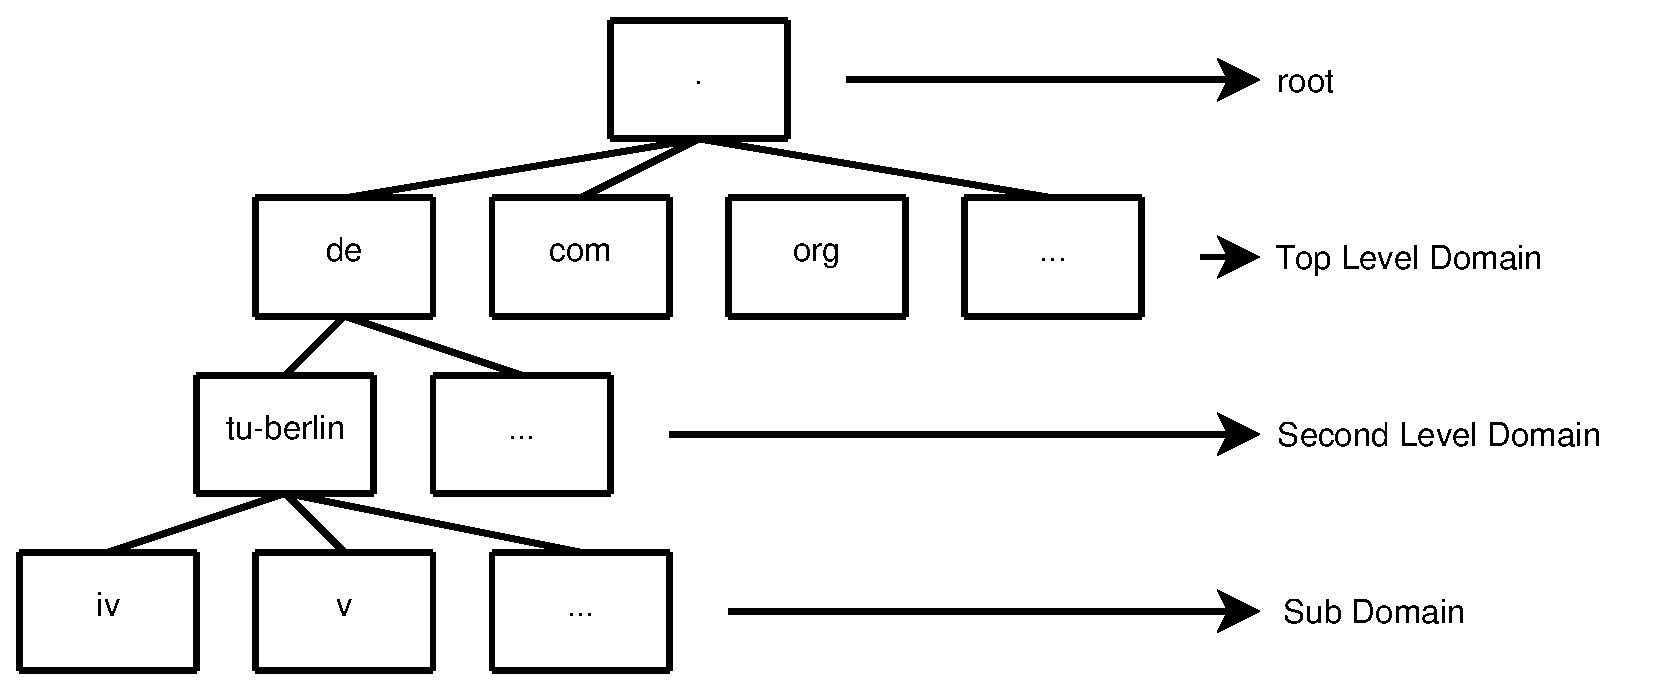
\includegraphics[width=0.8\textwidth]{dns}
\caption{Baumartige Struktur der DNS-Hierarchie}
\label{fig:dns}
\end{figure}

Diese Namensaufl�sung, das hei�t die Zuordnung eines Domain-Namens zu einer IP-Adresse wird im Internet von den DNS-Servern durchgef�hrt. Die erste Anfrage eines Benutzers zu der IP-Adresse einer Domain geht zuerst einmal eine Anfrage an den DNS-Server des Providers. Sollte der keinen Eintrag zu dieser Domain haben, sendet er eine Anfrage an einen der 13 DNS-Root-Server.

Wie in Abbildung~\ref{fig:dns} zu sehen ist, ist dieser DNS-Root-Server der oberste Knoten eines Baumes - hier mit einem Punkt bezeichnet. Von dort aus wird nun rekursiv eine Anfrage gestartet. Der Domain-Name wird von rechts nach links aufgel�st, d.h. zuerst wird bei meinem Beispiel die \texttt{de}-Endung verfolgt, danach der Teil \texttt{tu-berlin} usw.. Bei jedem Schritt wird ein neuer DNS-Server nach der IP-Adresse gefragt. Sollte bei diesem Server kein Eintrag zu der Anfrage vorhanden sein, wird diese Anfrage an den n�chsten zust�ndigen DNS-Server weitergeleitet. Also beispielsweise sendet der DNS-Root-Server die IP-Adresse des DNS-Servers der Domain \texttt{tu-berlin.de}. Dieser hat m�glicherweise die IP-Adresse des gesuchten Web-Servers nicht eingetragen, sendet also nun die Anfrage weiter an den DNS-Server der Subdomain \texttt{iv}. Sp�testens hier sollte ein Eintrag f�r den Web-Server (\texttt{www.iv.tu-berlin.de}) dieser Domain vorhanden sein. Diese nun ermittelte IP-Adresse wird nun an den DNS-Server des Providers zur�ck gesendet, der diese wiederum dem anfragenden Benutzer mitteilt.

Die vermittelte Adresse kann der DNS-Server des Providers nun auch speichern. Dieses so genannte \textit{Caching} erlaubt eine schnellere Beantwortung der DNS-Anfragen. Sollte nun wieder eine Anfrage an den DNS-Server gehen, welche die Domain \url{www.iv.tu-berlin.de} aufgel�st haben m�chte, so kann dies schnell �ber die nun gespeicherte IP-Adresse geschehen. Diese Cache-Eintr�ge werden jedoch nach einer bestimmten Zeit, der TTL (Time-To-Live), wieder gel�scht, da es oftmals vorkommt, dass sich IP-Adressen �ndern und so dann evtl. eine falsche Antwort kommen w�rde.

Die zweite Methode ist die reversible Namensaufl�sung (\textit{Reverse Lookup}). Hierbei wird der umgekehrte Weg beschritten, n�mlich die Zuordnung des Domainnamens zu einer bestimmten IP-Adresse. Hierzu wird auf jedem DNS-Server eine \textit{Reverse Lookup Tabelle} eingerichtet. Diese Tabelle enth�lt Eintr�ge, nach denen jeder IP-Adresse im Subnetz des verwaltenden DNS-Servers ein Domainname zugeordnet werden kann.

Jede Ebene der Referenzmodelle birgt Schwachstellen. Jedes System eines Netzwerks nutzt die Funktionen dieser Ebenen. Somit besteht die M�glichkeit, dass jedes System auch Teil eines Angriffs wird.

\subsection{Angriffsziele}
Nun muss �berlegt werden, welche Ziele ein Angreifer im Netzwerk haben kann. Welches Ziel steuert er an? Warum m�chte er gerade dieses Ziel angreifen? Ein Angriff hat auf unterschiedlichen Systemen auch unterschiedliche Auswirkungen, sowohl f�r das System selbst als auch f�r das Netzwerk, indem es integriert ist. Diese Arbeit differenziert Angriffe auf Router, Server und auf Endbenutzer.

\subsubsection{Router}
\label{sec:router}
Router sind Schnittstellen zwischen verschiedenen Netzwerken, deren Aufgabe darin besteht den Nachrichtenaustausch zwischen den Netzwerken zu gew�hrleisten. Die \textit{Destination Address}, also Zieladresse von IP-Paketen werden von Routern benutzt. Sie regeln das Weitersenden von eingehenden IP-Paketen aufgrund einer Routingtabelle. Eine solche Routingtabelle enth�lt zu jeder Ziel-IP-Adresse eines Nachrichtenpakets eine zugeh�rige Schnittstelle.
\begin{table}[htb]
\centering
\begin{tabular}{llll}
Destination Network & Netmask & Router & Metric\\
\midrule
192.168.0.0 & 255.255.255.0 & 192.168.0.1 & 1\\
245.133.2.0 & 255.255.255.0 & 245.133.2.1 & 1\\
135.22.0.0 & 255.255.0.0 & 135.22.0.1 & 2\\
135.22.0.0 & 255.255.0.0 & 135.22.1.1 & 3\\
\midrule
\end{tabular}
\caption{Beispiel einer Routingtabelle}
\label{tab:routingtabelle}
\end{table}

Wie in Tabelle~\ref{tab:routingtabelle} zu sehen ist, geschieht die Zuordnung anhand einer Maskierung der Zieladresse. Das bedeutet, dass die Ziel-IP-Adresse mit der Netzwerkmaske (Netmask) logisch mit UND verkn�pft wird und das Ergebnis mit der linken Spalte (Destination Network) verglichen wird. Stimmt nun eine der Adressen mit dem Ergebnis der UND-Verkn�pfung �berein, so wird das Paket an den n�chsten Router, der in der entsprechenden Zeile notiert ist weiter geschickt. Sollte es keine �bereinstimmungen geben wird das Paket verworfen.
\begin{figure}[htb]
\centering
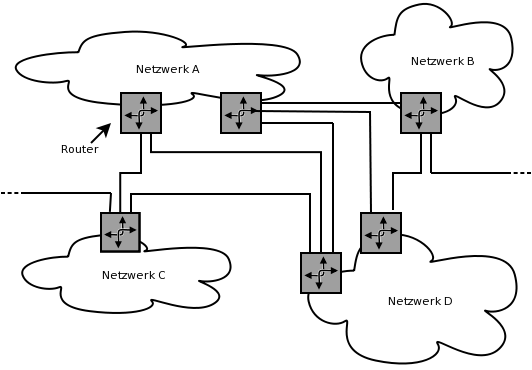
\includegraphics[width=0.8\textwidth]{internetskizze}
\caption{Grobe Skizzierung des Internets}
\label{fig:internetskizze}
\end{figure} 

M�glich ist auch, dass es zu einer Adresse mehrere Wege gibt. Dann entscheidet der Wert der letzten Spalte, die sog. Metrik �ber den n�chsten Router. Die Metrik beschreibt die Anzahl der Router, die auf dem Weg zum Ziel noch zu passieren sind. Je kleiner also dieser Wert ist, desto schneller wird das Paket vermeindlicherweise am Ziel ankommen.

Wie in Abb.~\ref{fig:internetskizze} zu sehen ist, kann das Internet grob gesehen als Zusammenschluss von vielen Netzen durch Router gesehen werden.

\subsubsection{Server}
Server sind in den einzelnen Netzwerken integriert. Server bieten Dienste an, die von vielen oder gar allen Nutzern im Internet abgerufen werden k�nnen. Diese Dienste sind z.B. HTTP, FTP oder Mail. Ein Webserver beispielsweise bietet Webseiten, die �ber einen Browser betrachtet werden k�nnen. Ein Mailserver bietet dagegen Dienste an, �ber die sich eMails verschicken und empfangen lassen.

Der Begriff "`Client"' bezeichnet den Nutzer der verschiedenen, von Servern angebotenen Dienste, also z.B. denjenigen, der den Browser bedient und damit Webinhalte der Webserver f�r sich nutzt.

\subsubsection{Endbenutzer}
Der Endbenutzer ist der Nutzer des Internets, der z.B. als Client bei einem Server Dienste, wie HTTP nutzt. Dieser sitzt zumeist an einem eigenen PC. Dieses 

\subsection{Der Angriff}
Die verschiedenen Ziele der Angreifer sind somit definiert. Nun stellt sich die Frage, was passiert, wenn das eine oder das andere ausgew�hlte Ziel gesch�digt wird und was ein potentieller Angreifer mit einer solchen Sch�digung erreichen m�chte. Darauf wird nun im Einzelnen eingegangen:
\begin{enumerate}
 \item \textbf{Router}: Ein Router ist, wie in Abb:~\ref{fig:internetskizze} zu sehen ist, ein empfindliches Bindeglied zwischen den Netzwerken. F�llt einer aus ist es eventuell noch nicht auff�llig, sobald aber mehrere Router ihren Dienst versagen kann dies schnell zu gr��eren Problemen f�hren. Wenn eine bestimmte Route �ber keinen der Router mehr zu erreichen ist, f�llt der gesamte Datenverkehr f�r diese Strecke aus. Jeder erdenkliche Dienst kann dann nicht mehr genutzt werden, da die Pakete, egal welcher Art, unterwegs auf jeden Fall verloren gehen.

 \item \textbf{Server}: Bei Servern ist die Situation nicht ganz so kritisch aber je nach Auftrag des Servers nicht minder wichtig. Der Ausfall eines oder mehrerer Server beeintr�chtigt nicht den gesamten Verkehr im Internet, jedoch nat�rlich den Verkehr, der auf die Server f�hrt.

So k�nnen z.B. St�rungen von Suchmaschinen-Servern dazu f�hren, dass die eine oder andere Suchmaschine nicht mehr zu erreichen ist. Dies k�nnte beispielsweise eine kriminelle Handlung eines Konkurrenten sein, der seine eigene Seite dadurch bevorteilen m�chte. Andererseits k�nnte ein Bank-Server in die H�nde eines Kriminellen geraten, der dann Zugriff auf die Konten hat.

 \item \textbf{Endbenutzer}: Der Endbenutzer ist zwar das kleinste aber auch das am wenigsten abgesicherte Ziel eines Angriffs. Die gro�en Systeme der Router und Server sind professionell �berwacht, w�hrend der kleine Anwender als Endbenutzer zumeist wenig Kenntnisse von Netzwerken und deren potentiellen Gefahren hat. Diese Rechner werden zumeist mit W�rmern und Viren angegriffen, die dann verschiedene Dinge ausl�sen.

Die Angriffe auf Endbenutzer sind zumeist noch die harmlosesten, da zum einen die St�rung eines einzelnen Rechners im Internet keine sonderlichen Auswirkungen hat und zum anderen bei einzelnen Benutzern nicht viel zu erreichen ist. Bekannt sind hier eher Schadprogramme, die z.B. die Daten des Benutzers l�schen oder seine Kontodaten ausspionieren.
\end{enumerate}
Oftmals werden solche Angriffe auf Server und Endbenutzer dazu genutzt um auf Schwachstellen aufmerksam zu machen. So genannte \textit{Hacker} versuchen mit den ihnen zur Verf�gung stehenden Mitteln in die Rechner einzudringen und oftmals harmlose Spuren zu hinterlassen, die eher l�stig als gef�hrlich sind.

Jedoch ist jegliche Art von Angriff als "`unerw�nscht"' einzustufen, da jeder die M�glichkeit aufzeigt, wo und auf welche Art und Weise auch gef�hrliche Angriffe vollzogen werden k�nnen. Es gibt Angriffe von au�en, also solche, bei denen der Angreifer nicht im eigenen Netzwerk sitzt. Demnach gibt es dann auch noch Angriffe von innen, die prinzipiell gef�hrlicher sein k�nnen, da die meisten Abwehrmechanismen gegen externe Angriffe wirken. Intern l�sst sich jedoch jegliche Manipulation leichter nach verfolgen und "`Gefahrenherde"' sind schneller erkannt und k�nnen bek�mpft werden, da der Administrator auf jeden Router, Server und Endrechner Zugriff hat. Dieser Zugriff erm�glicht die Auswertung verschiedenster Log-Dateien und somit das Nach verfolgen aller im Netzwerk gesendeten Pakete.

Zus�tzlich lassen sich Angriffe physischer oder virtueller Art unterscheiden. Verschiedenste Bedrohungen f�r Netzwerke, seien es interne Netzwerke oder das Internet werden im folgenden Abschnitt nun erl�utert.

\section{Bedrohungen}
Der folgende Abschnitt beschreibt Angriffe auf Router, Server und Endbenutzer und zeigt, was bei welchen Systemen zu Problemen f�hren kann und welche Auswirkungen dies haben k�nnte.

\subsection{(Distributed) Denial Of Service}
\label{sec:ddos}
Denial Of Service (abgek�rzt: DoS) ist eine Variante eines Angriffs, die im Grunde jedes Computersystem lahm legen kann. Somit k�nnen damit Server, Router und Endbenutzer gleicherma�en angegriffen werden. DoS bedeutet �bersetzt etwa "`au�er Betrieb setzen"'. Grob gesagt wird dieses Versagen durch eine Flut von Paketen erzeugt, die an die jeweilige Adresse des anzugreifenden Systems geschickt werden. Diese Flut bewirkt dann eine Belastung des Systems, welche im schlimmsten Fall zu einem Absturz f�hrt. Im weniger brisanten Fall wird nur eine bestimmte Komponente des Systems lahm gelegt. DoS kann aber nicht nur durch �berlast geschehen, sondern auch auf Implementierungsfehlern basieren. Das hei�t, dass durch Fehler im Programmcode beispielsweise der Serveranwendung gezielt gegen diese vorgegangen werden kann, was dann z.B. zum Absturz der jeweiligen Anwendung f�hren kann.

Man kann das Ziel eines solchen Angriffs grob in vier Punkte unterteilen:
\begin{enumerate}
 \item Absturz eines Systems
 \item Verhindern des Datenverkehrs zwischen zwei Systemen
 \item Belastung eines Netzwerks zur Verlangsamung der Geschwindigkeit und Verschlechterung der Produktivit�t
 \item Blockierung eines Systems. Gef�hrlicher als ein Absturz, da kein Neustart erfolgt
\end{enumerate}

Die �berflutung ist nat�rlich um so wirkungsvoller, je mehr Pakete bei dem "`Opfer"' ankommen. Hier gewinnt der Zusatz \textit{Distributed}, also \textit{verteilt}, an Bedeutung. Durch die Involvierung vieler, zumeist nichtsahnender Internetnutzer werden die Flut-Pakete von vielen PCs gleichzeitig zum Opfer geschickt. Dies l�sst sich z.B. durch Trojaner (siehe Abschnitt~\ref{sec:trojaner}) bewirken, durch die die Kontrolle eines fremden PCs m�glich ist. Durch diese Fremdkontrolle gelingt es dem Angreifer unbemerkt viele Pakete ans Ziel zu bringen. Unbemerkt in dem Sinn, dass der Absender nicht Angreifer ist, sondern mehrere unschuldige Dritte diesen Angriff durchf�hren.

\begin{figure}[htb]
\centering
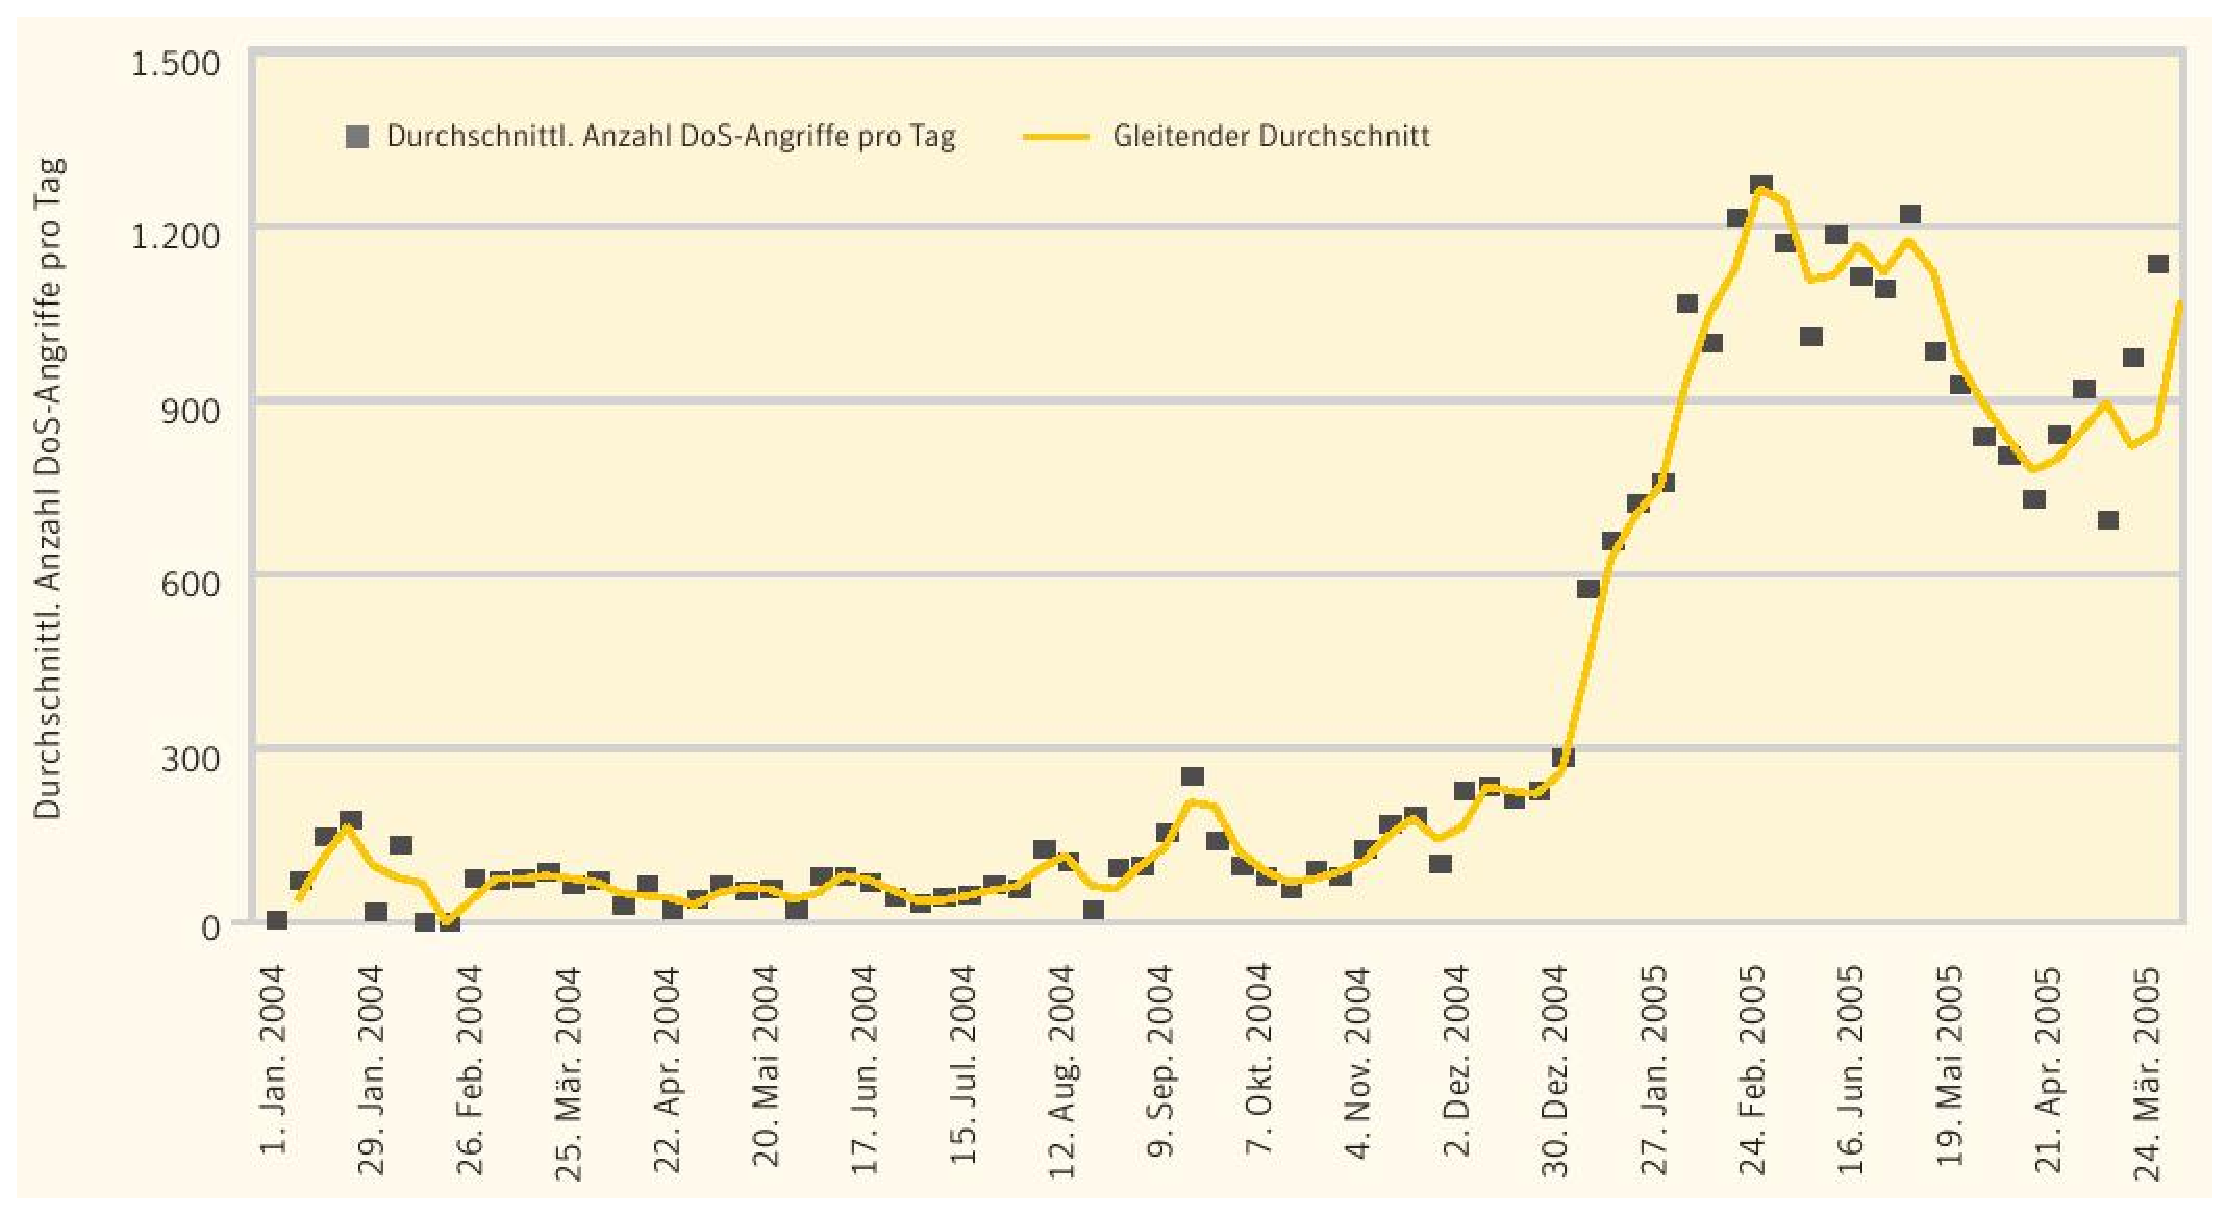
\includegraphics[width=0.8\textwidth]{dos}
\caption{Anzahl der DoS-Angriffe - Quelle: Symantec Band VIII\cite{symantec}}
\label{fig:dos}
\end{figure} 
Die Anzahl der DoS-Angriffe hat vor allem seit Anfang 2005 stark zugenommen. So hat sich die Anzahl der durchschnittlichen Angriffe pro Tag von ca. 200 auf ca. 1000 erh�ht.

Durch diese DoS-Methode k�nnen auch Router angegriffen werden und deren Belastungsgrenze bis aufs �u�erste ausgereizt werden. Ohne Schutzmechanismen w�re auch ein Router schnell mit so vielen Paketen �berfordert, bzw. w�rde sehr viele wichtige Pakete, die ihn passieren wegen Puffer�berlaufs verwerfen. Das w�rde das Internet im Ganzen blockieren, da nun die Sender immer und immer wieder versuchen werden ihre TCP-Pakete an den Empf�nger zu senden, jedoch beim Router scheitern. Wenn nun auch noch mehrere Router betroffen sind besteht auch nicht mehr die M�glichkeit einen anderen Weg zu suchen. Ein solcher Angriff auf Router ist sicher der effektivste aber zugleich auch schwierigste, da die Router der heutigen Generation sehr spezialisierte Systeme sind, die diese DoS-Attacken erkennen und bek�mpfen k�nnen.
%
% !!!!!!!!!!!! WIEEEEEEEEEEEEEEEEEE BEK�MPFEN !!!!!!!!!!!!!!!!!!!!!!!!!!!!!!!
%

Im folgenden werden nun ausschnittsweise verschiedene Varianten der DoS-Attacken erl�utert.

\subsubsection{SYN-Flooding/Land}
\label{sec:synflood}
Diese Methode nutzt den Verbindungsstatus einer TCP-Verbindung aus. Beim Aufbau einer solchen TCP-Verbindung wird, wie in Abschnitt\ref{sec:tcp} erw�hnt, ein Handshake-Mechanismus verwendet. Dieser kann nun gezielt zum Angriff genutzt werden.

Die \textit{Land-Attacke} realisiert dies nun, indem sie das SYN-Paket des Senders mit einer falschen Absenderadresse versieht. Das f�hrt nun dazu, dass der Empf�nger sein SYN/ACK-Paket an die falsche Adresse sendet und keine Antwort erh�lt.
\begin{figure}[htb]
\centering
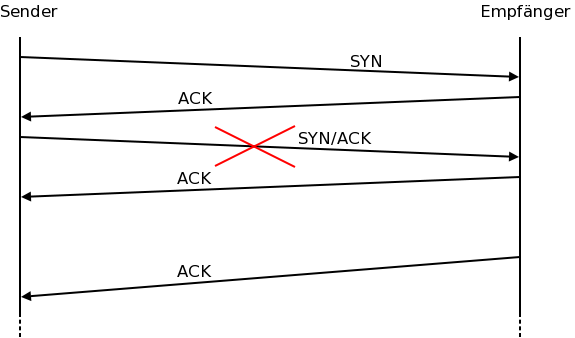
\includegraphics[width=0.8\textwidth]{handshake}
\caption{Handshake vor der TCP-Verbindung}
\label{fig:handshake}
\end{figure}
Das wiederum f�hrt dazu, dass der Empf�nger immer wieder versucht sein SYN/ACK-Paket zu senden, jedoch keine Antwort erh�lt. Dies geschieht so lange bis ein Timeout diese Versuche abbricht. Der Sender, also der Angreifer wird aber nicht nur ein SYN-Paket schicken, sondern gleich eine ganze Reihe von solchen Paketen.

\subsubsection{Ping of Death}
Diese Variante ist eine der einfachsten M�glichkeiten eines DoS-Angriffs. Hierbei wird die Fragmentierung von TCP ausgenutzt. Die Maximale Paketgr��e eines TCP-Paketes ist 65.535 Byte. Je nach Einstellung der Internetverbindung werden TCP Pakete fragmentiert, das hei�t in mehrere kleinere Pakete unterteilt und beim Empf�nger wieder zusammengesetzt.

Ein Offset-Wert bestimmt hierbei wann welches Paket anf�ngt. Durch Manipulation dieses Wertes des letzten fragmentierten Paketes wird erreicht, dass das gesamte Paket die maximale Gr��e �berschreitet. Wenn die zusammengesetzte Paketgr��e die Gr��e von 65.535 Byte �bersteigt gibt es einen Puffer-�berlauf und im ung�nstigsten Fall einen Absturz des empfangenden Rechners. Diese L�cke wurde jedoch mittlerweile bei nahezu allen g�ngigen Betriebssystemen geschlossen.

Ein ICMP-Echo-Requests w�re die einfachste Variante eines solchen Paketes. Mit einem \textit{ping}-Befehl k�nnen solche ICMP-Nachrichten versendet werden. Allerdings muss hierzu das regul�re \textit{ping} abge�ndert werden, da in der offiziellen Version die fehlerhafte Konstruktion eines solchen Paketes nicht gestattet ist.

\subsubsection{Smurf}
Bei einem Smurf-Angriff werden vom Angreifer sehr viele ICMP-Pakete an die Broadcast-Adresse eines Netzwerk geschickt, so dass jeder Rechner dieses Netzwerks diese Pakete erh�lt.

Der Angreifer tarnt seine Pakete nicht mit einer unbekannten Adresse sondern gibt als Absenderadresse die Adresse des Opfers an. Somit werden nun alle Antwortpakete dieses Broadcast-Netzwerks an das Opfer geschickt. Sollten also beispielsweise 1000 Rechner in diesem Netzwerk antworten und der Angreifer hat 1000 Pakete geschickt erh�lt das Opfer $1000 * 1000 = 1.000.000$ Antwort-Paket. Dadurch wird die Kapazit�t des Opfers voll ausgesch�pft und dieser kann nicht mehr andere Datentransfers durchf�hren.

\subsubsection{Teardrop}
Wie beim \textit{Ping of Death} nutzt auch diese Methode die Fragmentierung von gro�en TCP-Paketen aus. Jedoch wird hierbei keine �berl�nge der Pakete generiert, sondern die Fragmente �berlappen sich gegenseitig, so dass das Betriebssystem des angegriffenen Rechners mehr Ressources zum Zusammensetzen der Pakete belegt als es verkraften kann. Die Folge ist der Absturz des Systems.

Um einen DDoS-Angriffe starten zu k�nnen, m�ssen viele Rechner unter die Kontrolle des Angreifers gebracht werden. Um diese Kontrolle zu erreichen, werden Programme entwickelt. Diese Programme werden �ber W�rmer oder Trojaner verbreitet. Die Existenz eines solchen Trojaners auf einem PC kann den Zugriff auf diesen erm�glichen. 

\subsection{Trojaner}
\label{sec:trojaner}
Trojaner sind Programme, die zumeist �ber Dateianh�nge in eMails verbreitet werden. Sie haben meist "`harmlos"' klingende Namen. Diese Programme enthalten jedoch sch�dliche Komponenten. Der Begriff \textit{Trojaner} wurde aus der Mythologie des \textit{Tronjanischen Pferdes} �bernommen.

\subsection{Bots}
\label{sec:bots}
 Mit Trojanern ist es m�glich, den infizierten PC zu einem Bot werden zu lassen (Bots: Abk�rzung f�r das englische Wort f�r Roboter "`robots"'). Bots sind demnach infizierte PCs, die mit Hilfe der Trojaner dazu veranlassen werden k�nnen, bestimmte Dinge zu tun. Zumeist werden solche Bots dann genutzt, um den PC fernzusteuern. Sie k�nnen beispielsweise genutzt werden um DoS-Attacken (vgl. Abschnitt~\ref{sec:ddos}) auszuf�hren. Sie sind in der Lage viele Pakete zu generieren und abzuschicken.

Trojaner k�nnen auf Servern und Endbenutzersystemen ausgef�hrt werden und diese dann fernsteuern. Zumeist werden hier aber wohl die Systeme der Endbenutzer benutzt, da diese noch immer am wenigsten abgesichert sind und sich daher bestens f�r eine solche Infizierung und anschlie�ende Fernsteuerung nutzen lassen.
\begin{figure}[htb]
\centering
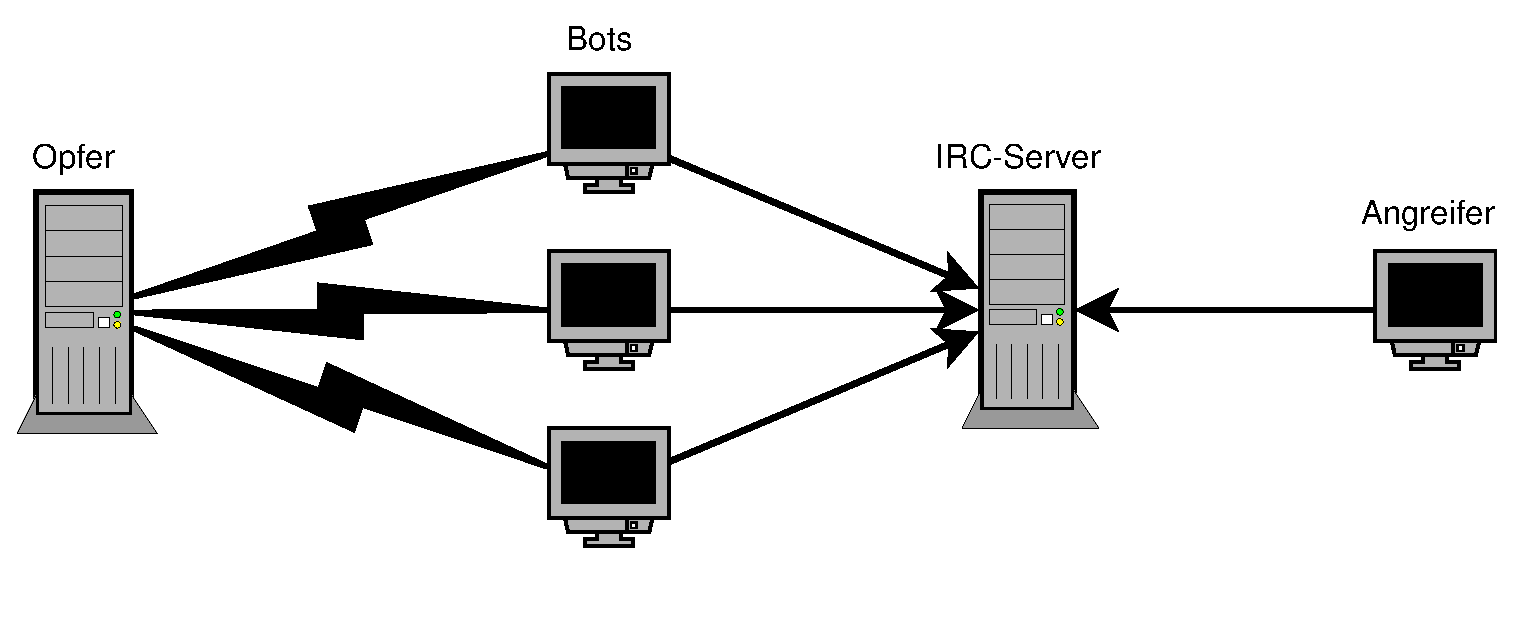
\includegraphics[width=0.8\textwidth]{botnet}
\caption{Darstellung eines typischen Botnetzwerks}
\label{fig:botnet}
\end{figure}

Die Fernsteuerung l�uft in der Regel �ber ein IRC-Netzwerk. IRC (\textit{Internet Relay Chat}) ist ein Protokoll zur textuellen Kommunikation, dem sogenannten \textit{Chat}. Ein IRC-Server besitzt mehrere Chatr�ume, sog. \textit{Channels}, denen IRC-Clients beitreten k�nnen. Innerhalb eines Chatraums k�nnen dann beliebige Textnachrichten ausgetauscht werden. Diese Prinzip machen sich nun Angreifer zunutze. Jeder Bot tritt einem bestimmten, vom Angreifer gew�hlten Chatraum bei. Somit besitzt der Angreifer die M�glichkeit, seinen Bots mittels Textnachrichten Befehle zu erteilten, die beispielsweise einen SYN-Flood Angriff einleiten.
\begin{figure}[htb]
\centering
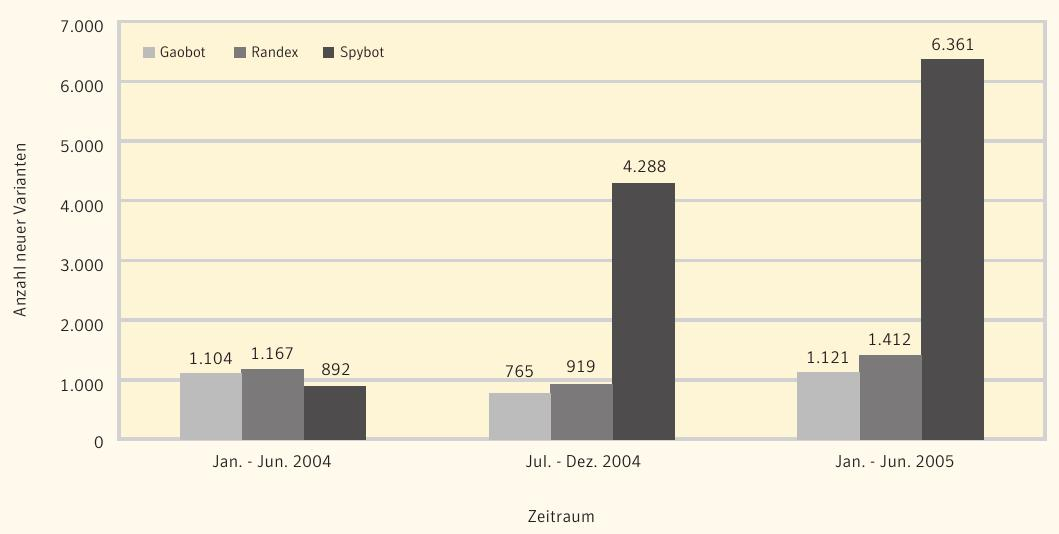
\includegraphics[width=0.8\textwidth]{bots}
\caption{Anzahl der Bots - Quelle: Symantec Band VIII\cite{symantec}}
\label{fig:bots}
\end{figure}

Die Anzahl der Bots ist in dem Zeitraum von Anfang 2004 bis Anfang 2005 gestiegen (siehe Abbildung~\ref{fig:bots}). Die Anzahl der Bots und die Anzahl der DoS-Angriffe h�ngen wohl zusammen, denn solche Bots eignen sich gut daf�r verteilte DoS durchzuf�hren, d.h. ein so genanntes Bot-Netzwerk aufzubauen, welches dann gemeinsam mehrere PC dazu missbraucht ein ausgesuchtes anderes System im Internet, sei es einen Server, einen Router oder einen anderer Endbenutzer zu attackieren.

\subsection{W�rmer}
W�rmer sind eigenst�ndige Programme, die �ber L�cken im Betriebssystem auf einen Rechner gelangen k�nnen. Diese L�cken entstehen durch offene Ports, d.h. durch Schnittstellen im Betriebssystem, die f�r bestimmte Dienst genutzt werden. Auch W�rmer k�nnen so programmiert sein, dass sie dem Entwickler eine Fernkontrolle erm�glichen. 

\subsection{Viren}
Viren sind kleine Programmst�cke. Sie k�nnen sowohl in einer Datei oder im Speicher befinden. Viren sind nicht eigenst�ndig, ben�tigen immer ein Medium, welches sie "`infizieren"'.
 
Viren sind in der Lage sich selbst zu verbreiten, indem sie sich beispielsweise �ber das Adressbuch des "`befallenen"' PCs an viele weitere PCs per eMail verschicken.
\begin{figure}[htb]
\centering
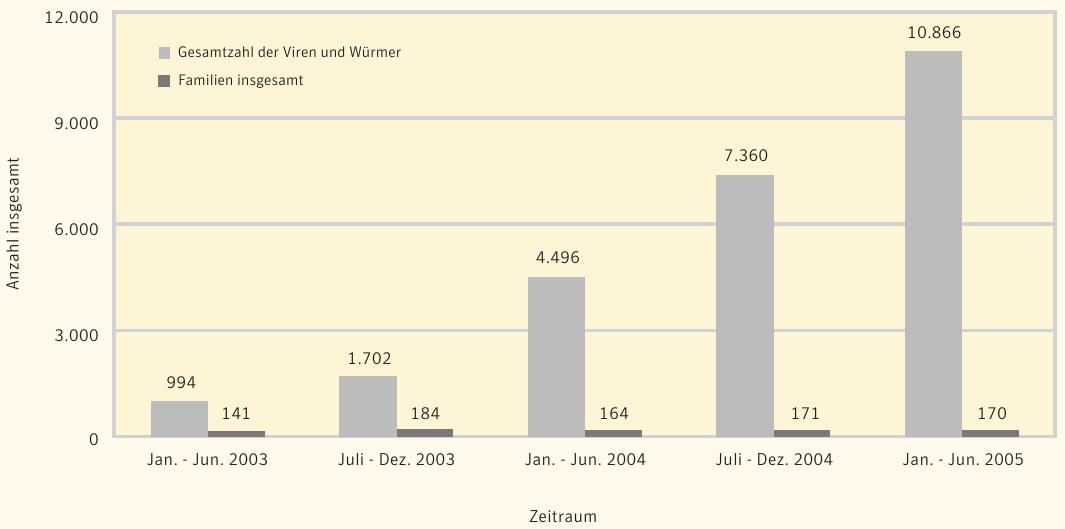
\includegraphics[width=0.8\textwidth]{viren}
\caption{Statistik zum Virenzuwachs - Quelle: Symantec Band VIII\cite{symantec}}
\label{fig:viren}
\end{figure}

Die Zahl der Viren hat sich, wie in Abbildung~\ref{fig:viren} zu sehen ist, innerhalb von 2 Jahren, von Januar 2003 bis Januar 2005 verzehnfacht. 

Hierbei hat sich die Anzahl der Virenfamilien aber nicht merklich ver�ndert. Viren werden aufgrund ihrer Struktur und arbeitsweise in verschiedene Klassen, sogenannte Virenfamilien aufgeteilt. Diese Anzahl der Virenfamilien schwankt um einen Wert von ca. 160. Das bedeutet, dass die Viren nur dadurch vermehrt auftreten, dass der Virencode leicht abge�ndert wird, so dass Virenscanner ihn nicht mehr erkennen. So m�ssen Virenscanner immer wieder aktualisiert werden und die st�ndigen Variationen in Ihre Datenbanken aufnehmen.

Viren, W�rmer und Trojaner k�nnne befallene Rechner sch�digen, indem sie beispielsweise bestimmte Verzeichnisse l�schen. Somit kann ein irreparabler Schaden angerichtet werden. Manchmal bel�stigen solche Programme auch nur den Nutzer, wie z.B. durch das Herunterfahren des Systems. Diverse Sicherheitsmechanismen, wie Dateirechte und Firewalls (siehe Abschnitt~\ref{sec:firewall}) oder Antivirenprogramme (Abschnitt~\ref{sec:antiviren}) gew�hren Schutz. Jedoch gibt es immer wieder L�cken, die solche Schutzma�nahmen unwirksam machen.

\subsection{Bedrohungen mittels des DNS-Protokolls}
Das DNS-Protokoll (siehe Abschnitt~\ref{sec:dns}) ist f�r die Vereinfachung der Navigation durch die Vielzahl der Server weltweit ein sehr wichtiges Protokoll. Sollte dieses ausfallen oder anderweitig durch einen Angriff gest�rt sein, so lassen sich, je nach Ausma� des Angriffs viele Server nicht mehr �ber ihre Domain-Namen erreichen. Die Server sind zwar intakt und auch zu erreichen, jedoch nur direkt �ber ihre IP-Adresse. So lie�e sich \texttt{www.iv.tu-berlin.de} nur noch �ber \texttt{130.149.16.12} erreichen.

Die Bedeutung des DNS-Protokolls f�hrt auch zu indirekten Angriffsm�glichkeiten. Durch Methoden, die die Funktionalit�t des DNS-Dienstes ausnutzen, lassen sich beispielsweise falsche Eintr�ge in DNS-Servern platzieren. Diese Eintr�ge k�nnen zur Folge haben, dass Domainnamen falsch aufgel�st werden.

\subsubsection{Cache Poisoning}
Beim \textit{Cache Poisoning} wird ein anzugreifender DNS-Server so manipuliert, dass er auf eine Anfrage an einen DNS-Root-Server eine falsche Antwort erh�lt. Das DNS-Protokoll nutzt als alleinige Authentisierung eine 16-Bit gro�e ID, die \textit{Transaction-ID}. Sollte es dem Angreifer gelingen diese ID zu erraten, dann kann er das Antwortpaket f�lschen.

Die ID ist aber nicht alleine n�tig, um falsche Pakete zu senden. Der UDP-Port des DNS-Servers ist ebenso n�tig. Theoretisch w�re es m�glich, dass jede einzelne Anfrage �ber einen anderen Port gesendet wird. Dies wird aber in den aktuellen BIND Versionen nicht praktiziert (BIND ist der DNS-Server, welcher am h�ufigsten verwendet wird - Berkley Internet Name Domain).

So ist es also m�glich, dass der Angreifer mittels einens eigenen DNS-Servers manipulieren kann. Hat er also Kontrolle �ber einen DNS-Server, so kann er an den zu attackierenden DNS-Server eine Anfrage schicken, die die Aufl�sung des Domainnamens eines im Netz des Angreifers befindlichen Hosts enth�lt. Der angfragte DNS-Server wird dann wiederum eine Anfrage an den DNS-Server des Angreifer schicken, da der angefragte Host auf diesem Server eingetragen ist. Dieser Anfrage kann der Angreifer nun den von BIND benutzen Source-Port entnehmen und ihn f�r seine gef�lschten Antworten benutzen.

Das letzte n�tige Detail ist die Source-IP-Adresse, d.h. die IP-Adresse des zust�ndigen Nameservers. Diese ist bekannt und es ist kein Problem mehr Antwort-Pakete zu erstellen, welche die korrekte Source-IP-Adresse, den korrekten Source-Port und eine generierte ID, sowie die gef�lschte Antwort des Nameservers enthalten.

Eine besonders effiziente Art des \textit{Spoofings}, d.h. des Versendens von Paketen mit falschem Absender und manipuliertem Inhalt, ist die \textit{Geburtstags-Attacke} (Birthday-Attack), benannt nach dem Geburtstagsparadoxon:
\begin{quotation}
\textsc{Die Wahrscheinlichkeit, dass aus einer Gruppe von 23 Leuten mindestens zwei am gleichen Tag Geburtstag haben, ist gr��er als $0,5$.}
\end{quotation}
Dieses mathematische Ph�nomen nutzt nun der Angreifer. Hierbei wird die Fragestellung umformuliert. Bei der Geburtstags-Attacke ist nun die Frage, wieviele Anfragen und Antworten m�ssen gesendet werden, damit mit einer Wahrscheinlichkeit von �ber $0,5$ mindestens eine Antwort und eine Anfrage dieselbe  \textit{Transaction-ID} besitzen? Die Antwort auf diese Frage liefert folgende Formel:
$$P = 1 - (1 - \frac{1}{t})^{\frac{n * (n-1)}{2}}$$
Laut dieser Formel\cite{stewart} l�sst sich die Zahl der Pakete bestimmen. Es sind $n = 302$ Pakete, die n�tig sind, um bei $t = 65535$ m�glichen IDs eine Wahrscheinlichkeit von $P > 0,5$ zu erhalten.

Um nun seine Attacke mit m�glichst gro�er Wahrscheinlichkeit zu starten, sendet der Angreifer nun also 302 Anfragen an den anzugreifenden DNS-Server. Gleichzeitig werden ebensoviele manipulierte Antworten gesendet und der eigentlich zust�ndige Nameserver mit einer DoS-Attacke blockiert, so dass er nicht so schnell die korrekte IP-Adresse liefern kann. Jede dieser manipulierten Antwort-Pakete enth�lt eine andere generierte ID. Somit erreicht der Angreifer sein Ziel mit einer Wahrscheinlichkeit von etwa $50\%$. Sollte n�mlich nun die ID der gef�schten Antwort mit der, der erwarteten Antwort �bereinstimmen, so wird die Antwort f�r "`wahr"' empfunden und ein Eintrag im DNS-Cache vorgenommen, der die falsche IP-Adresse enth�lt. Dies h�lt nun solange an, bis der Timer abl�uft, der in dem manipulierten Antwortpaket als TTL-Feld (Time-To-Live) gegeben war.

Beim einfachen DNS Spoofing, w�rde die gleiche Paketanzahl zu einer Wahrscheinlichkeit von $\frac{302}{65535} = 0,0046$ f�r einen erfolgreichen Angriff f�hren. Bei einfachen Spoofing werden auf eine einzelne Anfrage mehrere Antworten mit unterschiedlichen IDs gesendet. Wie aber zu sehen ist, ist diese Methode weit ineffizienter als die Geburtstags-Attacke.

Wenn nun ein Client eine Anfrage an den DNS-Server sendet und nach der IP-Adresse der soeben manipulierten Domain fragt, so wird er eine falsche Antwort bekommen und auf einen anderen Server geleitet, als gew�nscht war.

\subsubsection{DNS Amplification}
Bei dieser Variante wird nicht der DNS-Server als eigentliches Ziel benutzt, sondern als Angreifer mi�braucht. Es wird ausgenutzt, dass bei DNS auf kurze Anfragepakete (60 Byte) lange Antwortpakete folgen. Diese k�nnen bis zu 4000 Byte gro� sein\cite{dnsamplification}, so dass der sogenannte Verst�rkungsfaktor mit $\frac{4000}{60}\approx67$ ziemlich hoch liegt. Somit ist es m�glich, durch gezielte Anfragen einen DNS-Server dazu zu veranlassen, Antwortpakete an einen anzugreifenden Dritten zu senden. Dazu wird in denen den Anfragepaketen die IP-Adresse gespooft.

\subsubsection{Phase Space Analysis Spoofing}
Die Geburtstags-Attacke kann mit einer Analyse der generierten Transaction-IDs noch verbessert werden. Da die IDs mit Pseudo Zufallsgeneratoren erzeugt werden, besteht die M�glichkeit f�r den Angreifer, die Schw�chen dieser Generatoren zu nutzen. Bei der Analyse einer Reihe von generierten IDs ist zu sehen, dass etwa bei BIND 8.4.3 ein gro�er Bereich von Zahlen gar nicht generiert wird\cite{stewart}. So kann durch Ausschluss dieser Zahlen die Wahrscheinlichkeit des korrekten Ratens einer ID nochmals erh�ht werden.

Neuere BIND Versionen und andere DNS-Server, wie \textit{djbdns}\footnote{\url{http://cr.yp.to/djbdns.html}}, benutzen bessere Generatoren f�r ihre Zufallszahlen\cite{stewart}, sind dadurch aber nicht gesch�tzt, auch wenn die Wahrscheinlichkeit eines erfolgreichen ID-Ratens sinkt.

Die falsche Aufl�sung von Domainnamen ist eine Bedrohung �ber das DNS-Protokoll. Diese Protokoll befindet sich in der Applikationsebene. Auf der Netzwerkebene besteht die M�glichkeit �ber das Routing, Pakete falsch zu vermitteln.  

\subsection{Bedrohungen �ber Routing Protokolle}
Bei Angriffen auf das Routing k�nnen Router so get�uscht werden, dass sie falsche Routinginformationen in ihre Routing-Tabelle aufnehmen. Diese falschen Routinginformationen k�nnen Angreifer nutzen. Beispielsweise k�nnte erreicht werden, dass alle Pakete, die eigentlich zu Router XY gelangen sollten, beim Angreifer ankommen. So kann er spionieren und sogar f�lschen, d.h. die Daten ver�ndert an ihr eigentliches Ziel weiterleiten. Diese Methode wird im allgemeinen als \textbf{Man in the Middle}-Methode bezeichnet.

\subsubsection{ARP}
Die einfachste Methode bietet ARP. Es ist zwar nicht direkt ein Routing-Protokoll hilft aber dabei, dass Pakete ihren Empf�nger erreichen. Das \textit{Address Resolution Protocol} ist dazu da, IP-Adressen MAC-Adressen zuzuweisen. Jede IP-Adresse hat eine eindeutige MAC-Adresse, welche f�r die Adressierung im Link-Layer wichtig ist. Mit ARP kann der Angreifer einfach eine Anfrage eines Senders nach der MAC-Adresse einer bestimmten IP mit seiner eigenen MAC-Adresse beantworten. Die IP bleibt zwar die gleiche, aber auf dem darunter liegenden Link-Layer (z.B. Ethernet) ist die Adresse eine falsche. So bekommt nun der Angreifer alle Pakete gesendet 

\subsubsection{RIP}
Das erste weit verbreitet eingesetzte Routing-Protokoll war RIP. Es arbeitet so, dass jeder der Router seine ihm bekannten Routen und deren Metrik, also die Anzahl der Hops bis zu einem bestimmten Ziel an alle Router seiner Domain schickt. Es handelt sich bei RIP um ein \textit{Distance-Vector-Protocol}. Die Domain ist im Falle von RIP v1 eine Broadcast-Domain, im Falle von RIP v2 eine Multicast-Domain. So kann einen Angreifer einfach die Route zu seinem Rechner mit einer sehr kleinen Metrik versehen und schon werden alle Pakete an ihn geschickt. Dieses Protokoll findet allerdings kaum noch Anwendung.

\subsubsection{EIGRP}
Heute wird eher das EIGRP benutzt (Enhanced Interior Gateway Routing Protocol). Wie der Name schon preisgibt, handelt es sich um ein internes Protokoll, welches f�r die Verst�ndigung der Router innerhalb eines autonomen Systems benutzt wird. Ein autonomes System bezeichnet ein Teilnetzwerk, was unter einer administrativen Verwaltung steht. Es ist ein Cisco\texttrademark-eigenes Protokoll, eine Erweiterung von IGRP und f�llt auch in die Klasse der \textit{Distance-Vector-Protocols}. Die Routingentscheidung wird nun aber nicht mehr nur durch die Anzahl der Hops, sondern auch �ber Parameter, wie Paketlaufzeit, Bandbreite, Verf�gbarkeit und Auslastung von Verbindungen bestimmt\cite{routing}. Genau wie RIP 2 arbeitet EIGRP �ber Multicast, d.h. auch bei EIGRP kann der Angreifer mith�ren und auch selbst konstruierte Routinginformationen an einen Router senden. Dieser sorgt dann daf�r, dass alle anderen auch dieses Update durchf�hren.

Wie RIP v2 bietet auch EIGRP einen MD5-Hash-Algorithmus zur Wahrung der Integrit�t von Paketen (siehe Abschnitt~\ref{sec:schluessel}. Es verhindert jedoch nicht, dass fr�her kopierte Update-Pakete zu einem sp�teren Zeitpunkt nochmal vom Angreifer gesendet werden k�nnen und das Routing beeintr�chtigen, falls dieses Update nicht mehr g�ltig ist.

\subsubsection{Protokollunabh�ngig}
Auch das Einspeisen von Routinginformationen zu nicht zugewiesenen Adressbl�cken stellt ein Problem dar. So sind von der IANA (\textit{Internet Assigned Numbers Authority}) Bereiche von IP-Adressen als "`nicht vergeben"' deklariert. Solche Adressen werden von DoS-Angreifern gerne als Source-IP-Adresse in den \textit{gespooften} Paketen verwendet. Wenn das Angriffsziel nun von einer DoS-Attacke getroffen wird und Antworten an diese "`nicht vergebene"' Adresse zur�ck schickt, so sind die Router meist so konfiguriert, dass sie Pakete mit einer solchen Ziel-Adresse verwerfen. Sollte aber nun in der Routingtabelle ein Eintrag zu einer solchen, eigentlich nicht vergebenen Adresse existieren, so w�rden die Pakete nicht verworfen. Diese Antwortpakete k�nnten nun an einen Dritten geleitet werden und somit eine weitere DoS-Attacke ausl�sen.

Ein weiteres Problem auch die "`Monokultur"' im Bereich der Routerkonstrukteure. Cis\-co\texttrademark~besitzt einen Markanteil von ca. $75\%$\cite{cisco} im Bereich Internet Backbone Routing. Durch ein einzelnes Problem bei der Software der Router von Cisco\texttrademark~ist es f�r Angreifer m�glich gleich gro�e Teile des Internets zu gef�hrden. Beispiele f�r Probleme auf Cisco Routern finden sich auf \textit{Security Focus}\footnote{\url{http://www.securityfocus.com}}. So lie� sich mit einfachen Mitteln Zugang zu Cisco Router erreichen\cite{ciscoexploit} oder �ber geschickte Ausnutzung des SNMP-Protokolls(\textit{Simple Network Managment Protocol}) Datenverkehr �ber gew�nschte eigene Routen umleiten\cite{ciscosnmp}.

Insgesamt bilden Angriffe auf das Routing eine Gefahr auf unterster Ebene. Durch solche Angriffe lassen sich ganze Firmennetzwerke in ihrem Betrieb beeintr�chtigen. Ebenso gro� ist die Gefahr von Spionage und F�lschung. So k�nnen �ber manipulierte Routen Datenpakete an Dritte geschickt werden, kopiert und auch ver�ndert werden, wenn Schutzmechanismen, wie z.B. MD5-Verschl�sselung nicht genutzt werden. 

Unterhalb der Netzwerkebene, in der die Funktionalit�t des Routings enthalten ist, existiert nur noch die Host-to-Network Ebene. Auch auf dieser Ebene k�nnen Netzwerkstrukturen bedroht werden.

\subsection{Bedrohungen der Physikalischen Infrastruktur}
Neben den virtuellen Angriffen, d.h. den Angriffen �ber entfernte Rechner auf die wichtigen Protokolle, gibt es aber nat�rlich auch Angriffe physikalischer Natur. Sei es durch mutwillige Zerst�rung durch Kriege oder Anschl�ge oder durch nat�rliche Einfl�sse, wie Erdbeben oder �hnliches.

Das Internet als Ganzes ist vom Grundkonzept her sehr robust. Ausf�lle einzelner Knoten lassen sich durch die Flexibilit�t des Netzes schnell ausgleichen. So werden Routerausf�lle von den Nachbarrouter schnell erkannt, die diese Information dann �ber die Routingprotokolle bekannt geben. Nicht zu verachten sind jedoch gewisse Schnittstellen und Leitungen, deren lokale N�he zueinander zu einem Problem werden k�nnen. So enden beispielsweise weite Teile der transatlantischen Datenverbindungen in den USA im Bereich New Jersey und Rhode Island. Alleine vier Kabel landen in Manasquan (New Jersey). Weitere in New York, Brookhaven, Bellport oder Green Hill\cite{icpc}.

Eine Katastrophe in diesem Bereich der Vereinigten Staaten, die die Datenkabel treffen w�rde, k�nnte die Datenverbindungen zwischen Europa und den USA sehr stark beeintr�chtigen. Es existieren zwar auch Leitungen von Amerika �ber Asien nach Europa, diese Kapazit�ten sind jedoch nur unzureichend\cite{Quelle!}. 
%% !!!!!!!!! QUELLLLLLLLLLEEEEEEEEEE!!!
Ein Ausbau dieser Verbindungen zwischen Asien und Europa k�nnte auch f�r Entlastung der Verbindung USA - Europa sorgen.

Ein weiterer Punkt sind die Peering-Points und Internethubs, die ebenfalls zentrale Knoten im Internet darstellen. �ber diese Knoten tauschen die gro�en Provider ihre Daten aus, so dass sehr viel Verkehr �ber diese Systeme geht.
Folgend werden ein paar zentrale Peering-Points genannt.
\begin{description}
 \item[DE-CIX] Deutscher Commercial Internet Exchange. An diesen Netzknoten sind zur Zeit 180 Autonome System angeschlossen\cite{decix}, knapp 41 Gbps durchschnittlicher Datenverkehr zeugen von hohem Durchsatz, denn fast alle Provider sind mit diesem Knoten verbunden

\item[LINX] London Internet Exchange. Er ist Europas gr��ter Peering-Point mit ca.\break 100 Gbps\cite{linx} durchschnittlichem Datenaufkommen.

\item[NYIIX] New York International Internet Exchange, mit etwa 12 Gbps Durchsatz\cite{nyiix}.

\item[AMS-IX] Amsterdamer Internet Exchange - 41,7 Gbps durchschnittlicher Durchsatz\cite{amsix}

\item[EQUINIX] 81 Gbps durchschnittlicher Durchsatz, kombinierter Verkehr von 5 gro�en Knoten innerhalb der USA\cite{equinix}
\end{description}
Dies ist nur eine begrenzte Auswahl. Es gibt zwar noch ein paar Peering-Points mehr, diese haben jedoch viel weniger Daten zu verarbeiten und zu vermitteln. Der l�ngerfristige Ausfall des \textit{DE-CIX} w�re sicherlich gut zu sp�ren. Wenn dann noch ein weiterer alternativer Peering-Point in Deutschland ausfallen w�rde k�nnte es schon zu gr��eren Problemen kommen. Mit einer solchen Alternative w�re ein Ausfall des \textit{DE-CIX} noch auszugleichen\cite{heise}.

Es ist zu sehen, dass es viele M�glichkeiten gibt, Netzwerke anzugreifen. Es existieren viele Bedrohungen, die jeweils einer der Ebenen im Ebenenmodell zuzuordnen sind. Manche der Bedrohungen sind rein theoretischer Natur und haben noch nicht zu gro�en Problemen gef�hrt. Jedoch soll diese Arbeit aufkl�ren was m�glich ist und die Bedrohungen benennen. Es sind auch Bedrohungen dabei, die bereits zu gr��eren Ausf�llen auf Servern gef�hrt haben. Ein paar von diesen Ausf�llen werden im kommenden Absatz beschrieben.

\section{Angriffshistorie}
Diese Sektion beschreibt exemplarisch Angriffe auf HTTP-Server. Staatliche, wie auch 
kommerzielle Seiten sind in den vergangen Jahren immer wieder solchen Angriffen ausgesetzt gewesen. Diese Daten k�nnen dazu benutzt werden, f�r die Zukunft aus diesen Angriffen zu lernen.
\begin{description}
 \item[26. Mai 1999, FBI] Der erste DoS-Angriff, der �ffentlich diskutiert wurde war ein Angriff auf die Webseite des FBI\cite{zdnet}. Die US-Institution hatte nach einigen Angriffen auf US-Regierungscomputer eine Suche nach Personen der Hacker Gruppe "`Global Hell"' begonnen. Daraufhin wurde die Webseite des FBI von den Hackern ins Visier genommen. Mehrere Stunden wurde die Seite au�er Gefecht gesetzt, so dass das FBI erst einmal keine andere Wahl hatte, als die Seite vom Netz zu nehmen, um gr��eren Schaden abzuwenden.
 
\item[7. Februar 2000, Yahoo\texttrademark] Yahoo, mittlerweile ein gro�e b�rsennotierte Gesellschaft, wurde Anfang 2000 mit einer sehr gro�en DoS-Attacke lahm gelegt. Nach Angaben von GlobalCenter\texttrademark, dem Webhoster von Yahoo, wurde zur Angriffszeit ein Datenaufkommen von 1 GBit pro Sekunde gemessen\cite{news}.
%%%%% VERGLEICH
Zum Vergleich: An einem ...
%%% VERGLEICH
Diese Ausma� konnte der Server, trotz implementierter Filtermechanismen, die eine gewisse maximale Datenmenge garantieren sollten, nicht verkraften.
 
\item[8. Februar 2000, Amazon\texttrademark, Buy.com\texttrademark, CNN\texttrademark, and eBay\texttrademark] Nachdem ei\-nen Tag zuvor Yahoo Ziel eines DoS-Angriffs war, wurden an diesem Tag gleich mehrere gro�e Internetfirmen attackiert\cite{cnn}. Und genau, wie tagszuvor, war die riesige Menge an Datenaufkommen welche von hunderten oder gar tausenden Bots generiert wurde, von den Servern nicht zu bew�ltigen. So waren die Betreiber der Seiten gezwungen, ihre Inhalte f�r einige Stunden vom Netz zu nehmen. Auch am Tag danach wurden noch Webseiten wie ZDNet\texttrademark und E*Trade\texttrademark von einer Attacke betroffen\cite{news2}. Insgesamt wurde im Februar des Jahres 2000 das Thema \textit{DoS-Attacken} erstmals weltweit wahrgenommen. Viele kleine weitere Angriffe fanden noch statt, und Experten waren gefragt, mit welchen Ma�nahmen man sich gegen solche Angriffe wehren k�nne.
 
\item[21. Mai 2001 CERT] F�r die Dauer von zwei Tagen wurde eine der wichtigsten Firmen f�r Internetsicherheitsthemen aufgrund einer DDoS-Attacke vom Netz genommen. Und diesmal ist zu sehen, dass selbst Internetfirmen wie CERT (Computer Emergency Response Team), die sich um die Sicherheit im Netz sorgen, nicht sicher vor DoS-Angriffen sind.
 
\item[1. Februar 2004, SCO\texttrademark] Mit einem sich weit verbreitenden Wurm hat sich Ende Februar 2004 ein DDoS Angriff angek�ndigt, der die Softwareschmiede SCO treffen sollte. Schon Wochen vorher war bekannt, dass am 01.02.2004 ein gro�er Angriff auf die Webseite der Firma SCO wirken w�rde. Mit einem Wurm, der sich selbstst�ndig weiterverbreitete\cite{symantecmydoom}, wurden Trojaner installiert. Bei diesen war schon im voraus bekannt, dass sie f�r den Angriff auf SCO konzipiert wurden. Nach einer Analyse von Sophos\texttrademark, eines Internetsicherheitsunternehmens, war im Januar 2004 dieser Wurm mit dem Namen \textit{MyDoom}\cite{bsimydoom} mit einem Anteil von $25,1\%$\cite{sophos} an der weltweiten Virenverseuchung beteiligt. Jedoch konnte trotz dieses Wissens eine solche Attacke auf die Webseite nicht verhindert werden. Mehrere Tage wurde die Seite mit einer Datenflut �berh�uft. Die einzige Gegenma�nahme, die getroffen wurde, war den DNS-Eintrag zu l�schen, so dass der Server nur noch direkt �ber die IP-Adresse erreichbar war\cite{wikipediamydoom}.
 
\item[04. Oktober 2004, holl�ndische Regierung] Nicht nur kommerzielle Betreiber von Webseiten, sondern auch staatliche Seiten werden vermehrt Ziel von DoS-Attacken. Im Oktober 2004 wurden mehrere Server der holl�ndischen Regierung angegriffen. Nach Angaben von Regierungssprechern\cite{isn} waren jedoch nur �ffentliche Informationsseiten betroffen und keine sicherheitsrelevanten Seiten. Dieser Angriff erfolgte vermutlich nach Protesten gegen die Arbeit der Regierung und stand im Zusammenhang mit diesen Geschehnissen. Im Juni 2006 passierte �hnliches mit einem Regierungsserver der schwedischen Regierung. Auch dieser Webserver der Regierung mit informativem Inhalt wurde f�r einige Stunden au�er Gefecht gesetzt\cite{thelocal}, nachdem bereits einen Tag zuvor die Webseite der schwedischen Polizei von einer DoS-Attacke betroffen war.
\end{description}
Wie an diesen Beispielen zu sehen ist, hat es in der j�ngsten Vergangenheit zahlreiche Angriffe auf Computersysteme mit gesellschaftlicher Relevanz gegeben. Diese hier gew�hlte Zusammenstellung ist nur ein kleiner Ausschnitt aus der Historie der Angriffe. Um weitere Angriffe zu verhindern m�ssen Ma�nahmen getroffen werden, die den Angreifern entgegen wirken.

\section{Gegenma�nahmen}
Um Angriffen, wie z.B. Trojanereinschleusung oder DoS etwas entgegen zu wirken, m�ssen Ma�nahmen getroffen werden. Solche Gegenma�nahmen k�nnen sowohl direkt als auch indirekt wirken. Einige der klassischen Gegenma�nahmen werden in den folgenden Abschnitten einmal kurz erl�utert.

\subsection{Pr�ventive Ma�nahmen}
Pr�ventiv sind jene Ma�nahmen, die schon im voraus die Folgen eines Angriffs abschw�chen sollen. So kann durch derartige Ma�nahmen verhindert werden, dass Angriffe �berhaupt stattfinden, wodurch ein Einschreiten nicht vonn�ten ist.

\subsubsection{Firewalls}
\label{sec:firewall}
Eine Firewall ist im Idealfall ein zus�tzlicher, autonomer Rechner, der zwischen zwei Netzwerken installiert wird. So erreicht man, dass der gesamte Datenverkehr den diese Netzwerke austauschen, diese Firewall passieren muss. Solche Netzwerke bestehen im allgemeinen aus einem lokalen Netzwerk (LAN) und dem Internet. Diese Firewall ist nun dazu da, nach bestimmten Regeln, Pakete zu filtern. Somit kann das interne Netzwerk �ber die Firewall gesch�tzt werden. Durch die Filterung ist es beispielsweise m�glich, Rechnern aus dem Internet das Verbinden �ber ein "`unerlaubtes"' Protokoll mit einem internen Rechner zu verhindern.
\begin{figure}[htb]
\centering
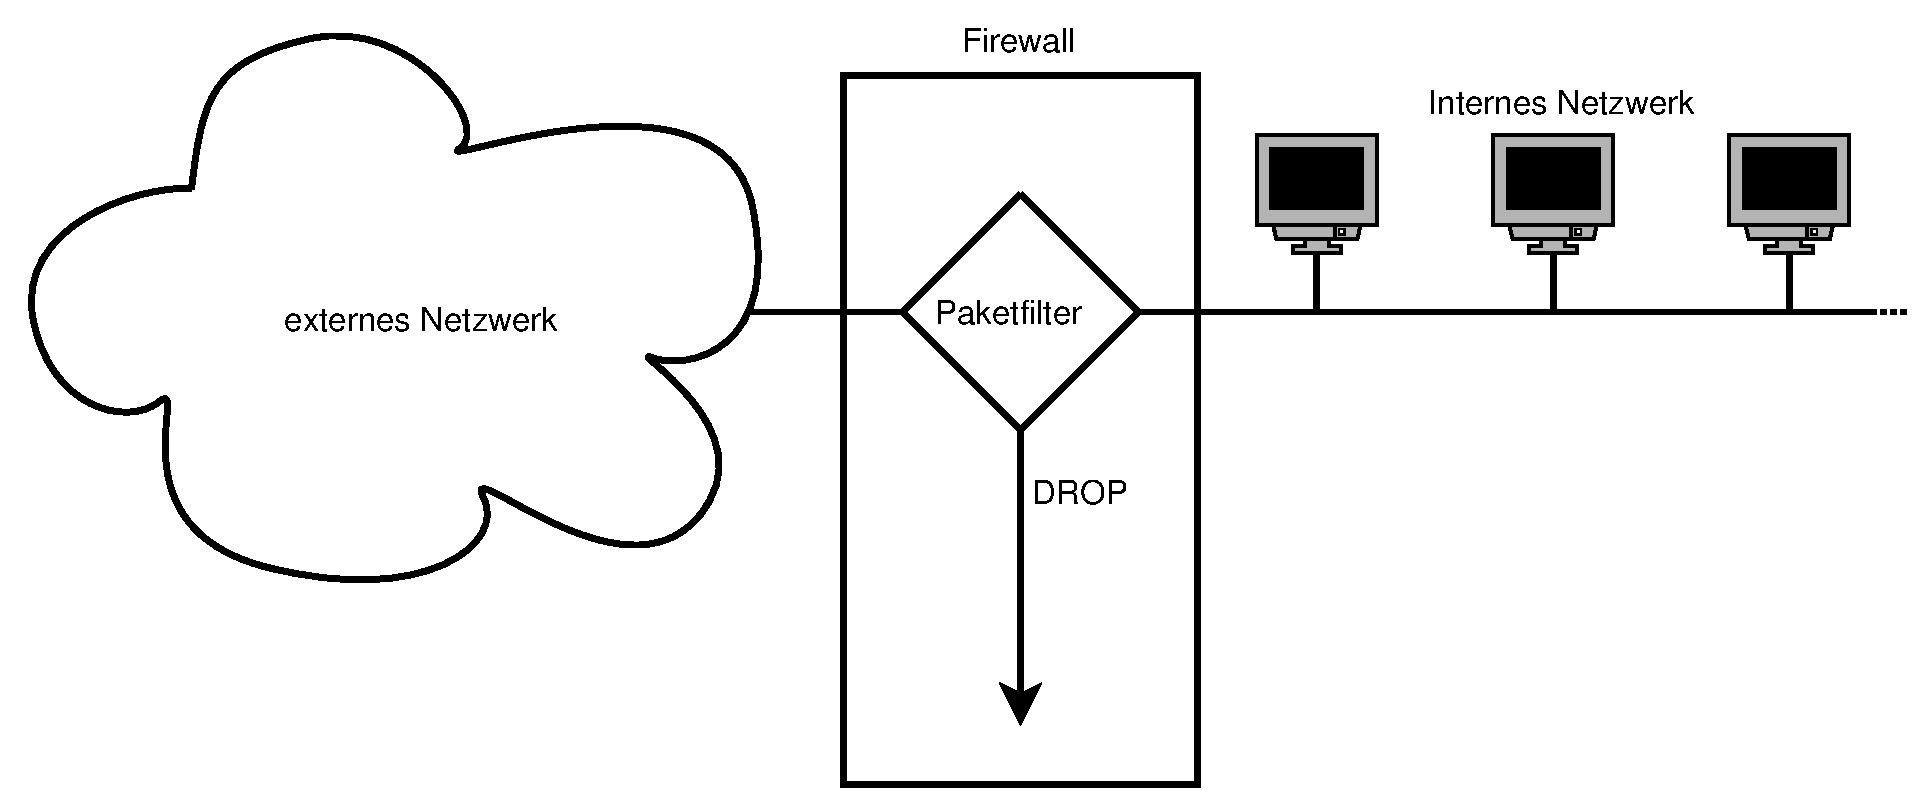
\includegraphics[width=0.8\textwidth]{firewall}
\caption{Grundprinzip einer Firewall}
\label{fig:firewall}
\end{figure} 

�ber eine Firewall kann also nach jeder in den Paketen oberhalb der IP-Ebene enthaltenen Informationen (Protokolltyp, Quellport, Zieladresse etc.) gefiltert werden. So lassen sich beispielsweise offene Ports von unsicher eingestuften Programmen vermeiden. Diese Ports sind zwar noch immer offen aber mit geeigneten Filterregeln nicht mehr von au�en zu erreichen. Es l�sst sich dadurch oberhalb der IP-Ebene der Zugang zum eigenen Netzwerk kontrollieren und beschr�nken, und somit Angreifern die Arbeit zumindest zu erschweren.

�ber eine Firewall k�nnen auch DoS-Attacken bek�mpft werden. Sollte eine DoS-Attacke stattfinden, ist es Aufgabe des Administrators, eine Signatur in der Flut der ankommenden Pakete zu erkennen. Diese erkannten Merkmale k�nnen dann der Firewall mitgeteilt werden, welche dann daf�r sorgt, dass Pakete mit diesen bekannten Merkmalen verworfen werden. So wird erreicht, dass die Paketflut zumindest nicht das interne Netzwerk erreicht. Die Firewall als solche kann nun aber trotz aller Vorsorge au�er Gefecht gesetzt werden.

\subsubsection{Verschl�sselung}
\label{sec:schluessel}
Mit der Verschl�sselung von Daten l�sst sich zwar nicht verhindern, dass ein System angegriffen und beispielsweise durch eine DoS-Attacke lahm gelegt werden kann. Jedoch kann hierdurch die Integrit�t von Daten gew�hrleistet werden.

Wie bei den Angriffen �ber Routingprotokolle schon erw�hnt, k�nnen Angreifer durch das Einschleusen falscher Routinginformationen das Routing so beeinflussen, dass viele Pakete das System passieren, welches sie unter Kontrolle haben. So ist es dann m�glich, Daten mitzulesen. Durch Verschl�sselung wird ein solches mitlesen unm�glich oder zumindest erschwert.

So k�nnten auch Routinginformationen ausgetauscht werden, ohne dass ein mitlesender Dritter Einsicht in die Topologie des Netzwerks nehmen k�nnte.

\subsubsection{Eingangsfilterung}
Die auch als \textit{Ingress Filtering}\cite{rfc2827ingressfiltering} bekannte Methode ist eine von Netzbetreibern, speziell ISPs (Internet Service Provider), verwandte Methode. Sie verhindert, dass IP-Spoofing, also das F�lschen der Absender IP-Adresse �ber ihr Netzwerk, m�glich ist. Mittels spezieller Paketfilter werden nur solche Pakete vom Kunden weitergeleitet, die als Absenderadresse auch wirklich die ihm zugeteilte Adresse enth�lt oder sich zumindest in dem providereigenen Subnetz befindet. Dadurch wird erreicht, dass das eigene Netz f�r Angreifer weniger attraktiv ist, da ihre Bots innerhalb dieses Netzwerks keine Quell-IP-Adressen f�lschen k�nnen. Somit sind sie dann sp�ter auch leichter aufzusp�ren.

Pr�ventive Ma�nahmen sind notwendig, jedoch nicht das einzige Mittel, welches zur Sicherung von Netzwerken eingesetzt werden sollte. Jede pr�ventive Ma�nahme hat Schw�chen die ausgenutzt werden k�nnen. Die pr�ventiven Ma�nahmen m�ssen durch Mechanismen erg�nzt werden, die auf Angriffe reagieren.

\subsection{Reaktive Ma�nahmen}
Die Erweiterung der Pr�ventionsma�nahmen sollten auf aktuelle Angriffe reagieren und deren Folgen mit geeigneten Ma�nahmen abmildern oder ganz verhindern.

\subsubsection{Intrusion Detection Systems}
\label{sec:ids}
Intrusion-Detection-Systeme bilden eine Einheit aus Anomalie- und Mustererkennung. Anhand bekannter Angriffe werden Signaturen erstellt, so dass mittels dieser Muster Datenstr�me analysiert und eingestuft werden k�nnen. Diese Methode funktioniert jedoch bisher nicht bekannten Angriffsmustern. Bei der Anomalieerkennung werden Datenstr�me mit einem "`Normalmodell"' verglichen. Werden Abweichungen oberhalb einer gewissen Toleranzschwelle erkannt, so k�nnen solche Datenstr�me als Angriffe eingestuft werden. Die Schwierigkeiten hierbei sind eine geeignete Wahl der Toleranzschwelle und die Definition des "`Normalmodells"'. Eine solches Intrusion-Detection-System kann leider auch missbraucht werden. So k�nnen Angreifer eine solche Anomalieerkennung durch gezielte Manipulation auch dazu bringen, legitimen Datenverkehr als Angriff zu interpretieren.

\subsubsection{Antivirenprogramme}
\label{sec:antiviren}
Neben der Firewall, die die Pakete kontrolliert und deren Zul�ssigkeit pr�ft, sind Antivirenprogramme dazu da, Viren, die den Weg an der Firewall vorbei geschafft haben zu erkennen und zu vernichten oder zumindest unter Quarant�ne zu stellen.

Antivirenprogramme auf Endbenutzersystemen kontrollieren st�ndig das Dateisystem und reagieren sofort bei Ver�nderungen. Das hei�t, sollte eine Datei abgelegt werden die f�r das Antivirenprogramm als gef�hrlich eingestuft wird, alarmiert es den Nutzer.

Antivirenprogramme k�nnen aber auch, z.B. auf Mailservern installiert werden. So k�nnen eventuell in Mails enthaltene Viren schon abgefangen werden, bevor sie das Endsystem erreichen.

Das Hauptproblem solcher Antivirenprogramme ist ihre Aktualit�t. Es k�nnen immer nur Viren erkannt werden, deren Struktur auch bekannt ist. Da aber t�glich, oft sogar st�ndlich, neue Viren entstehen besteht, das Problem darin, diese neuen Viren ebenso zu erfassen, wie "`alte Bekannte"'. Daher sind solche Antivirenprogramme immer mit Updatefunktionen ausgestattet, die z.B. eine t�glich Aktualisierung erm�glichen.

Antivirenprogramme entdecken auch Trojaner, die sich in Systeme einnisten. Diese k�nnen dann von Angreifern genutzt werden um DDoS-Attacken auf bestimmte Ziele zu starten. Da nach dem Start einer solchen Attacke die Verhinderung eines Ausfalls sehr schwer f�llt, ist also die Entdeckung und Beseitigung solcher Trojaner das prim�re Ziel zur Verhinderung von DDoS-Attacken. Aufgrund dieser Tatsache k�nnten Antivirenprogramme auch als \textit{pr�ventiv} gesehen werden.

Diese Gegenma�nahmen, aber auch andere, sollen dazu beitragen, dass ein Angriff auf Netzwerke oder einzelne Systeme gar nicht erst stattfinden oder zumindest erschwert werden. Trotzdem besteht die Gefahr, dass diese Ma�nahmen nicht wirken und Ausf�lle auftreten k�nnen.

\section{Ausfallpl�ne}
Bei allen Angriffen auf die Computersysteme der Welt, stellt sich doch nun die Frage, was passiert, wenn nun gr��ere, weitl�ufigere DoS-Attacken gestartet w�rden. Hier setzt nun meine Arbeit an. Im praktischen Teil meiner Ausarbeitung wird exemplarisch eine Angriffsvariante in einen Simulator integriert und analysiert, welche Auswirkungen in dem angegriffenen Netzwerk zu erkennen sind.

Prinzipiell ist der Angriff auf ein Netzwerk oder einen einzelnen Teilnehmer eines Netzwerkes leicht realisierbar. Sind gen�gend Bots im Internet "`platziert"', kann durch Aktivierung dieser Bots ein DDoS-Angriff gestartet werden.

Daher k�nnte es im Extremfall eines gro�en Netzwerkabsturzes n�tig sein, alternative Wege f�r eine Kommunikation zu nutzen. Da die Kritischen Infrastrukturen mehr und mehr von einem funktionierenden Nachrichtenaustausch abh�ngen, werden solchen Alternativen auch zunehmend gr��ere Beachtung geschenkt.

Eine dieser alternativen Nachrichtenwege w�re der \textit{Short Message Service} (SMS), welcher von Handynutzern zur Kommunikation mittels kleiner Textnachrichten genutzt wird. 

\subsection{SMS}
% http://www.smartmobs.com/archive/2004/10/06/dutch_governmen.html
% http://www.smsanalysis.org/
% auch sms betroffen von DoS
Der \textit{Short Message Service} ist ein Nachrichtensystem des GSM Mobilfunks, welches zum Austausch kleiner Textnachrichten mit einer L�nge von 140 (lateinischen) Zeichen entwickelt wurde. Um den Nachrichtenversand von einem PC �ber SMS zu erm�glichen, wurden sogenannte SMS-Gateways entwickelt. Mit diesen ist es m�glich, eine SMS (Kurzform f�r die Nachricht �ber den Short Message Service) via PC zu versenden. Somit k�nnte also der eMail-Versand �ber SMS alternativ geschehen. Dazu sieht die GSM-Spezifikation von SMS (3GPP TS 03.40\cite{gsmsms}) diese M�glichkeit in Punkt 3.8 vor. So kann also die beidseitige Umsetzung von SMS zu eMail �ber ein kompatibles Gateway realisiert werden.

Zudem muss der Empf�nger auch hinter einem SMS-Gateway sitzen, der die SMS empf�ngt und sie an den Empf�nger-PC weiterleitet. Dort muss dann die R�ckwandlung von SMS zu eMail erledigt werden.

\begin{figure}[htb]
\centering
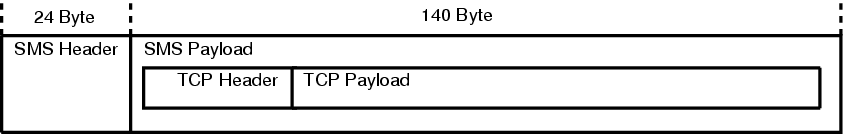
\includegraphics[width=0.8\textwidth]{sms}
\caption{Struktur eines SMS SUBMIT Paketes mit SSH Daten}
\label{fig:sms}
\end{figure}
Bei komplexerem Nachrichtenaustausch, z.B. einer verschl�sselten SSH-Sitzung, k�nnte eine Verbindung �ber bin�re Kurznachrichten, wie sie ebenfalls in der SMS-Spezifikation unter 9.1 zu finden ist, genutzt werden. Diese M�glichkeit wird heute auch schon genutzt, um beispielsweise Klingelt�ne auf Handys zu �bertragen. Eine Kurznachricht beinhaltet eine Payload von 140 Byte. Da SSH-Pakete eine variable L�nge haben, m�ssten diese entsprechend der SMS-Norm angepasst werden. In Abbildung~\ref{fig:sms} ist die grobe Struktur eines solchen Pakets zu sehen. SMS-SUBMIT-Pakete sind die Datenpakete, die von den \textit{Mobile Stations} an die \textit{Service Center}, d.h. von den Handys an die Netzbetreiber, gesendet werden.

Der Short Message Service ist nicht f�r gro�e Datenmengen ausgelegt. Mit HSCSD (\textit{High Speed Circuit Switched Data}), einer Erweiterung des GSM-Standards (3GPP TS 02.34\cite{gsmhscsd}) , ist eine Datenrate von maximal 57,6 kbit/s m�glich. Dies reicht f�r eine einfache Verbindung, um beispielsweise Textdaten zu versenden, aus.

\subsection{UMTS}
Wenn eine schnellere Datenverbindung vonn�ten ist, k�nnte auch UMTS (\textit{Universal Mobile Telecommunication System}), die neueste mobile Daten�bertragungstechnik, verwendet werden. UMTS bietet eine �bertragungsrate von bis zu 2 Mbps\cite{gsmumts}. Diese M�glichkeit ist daher f�r gro�e Datenvolumen gegen�ber SMS/GSM vorzuziehen.

\subsection{Alternativwege}
Sowohl �ber SMS als auch �ber UMTS w�re eine Datenverbindung m�glich, ohne vom Backbone des Internets abh�ngig zu sein. Dazu m�sste ein Gateway installiert werden, welches bei einem Ausfall der Verbindung zum Internet, wie es in Abbildung~\ref{fig:umtsgateway} zu erkennen ist, zwischengeschaltet wird.
\begin{figure}[htb]
\centering
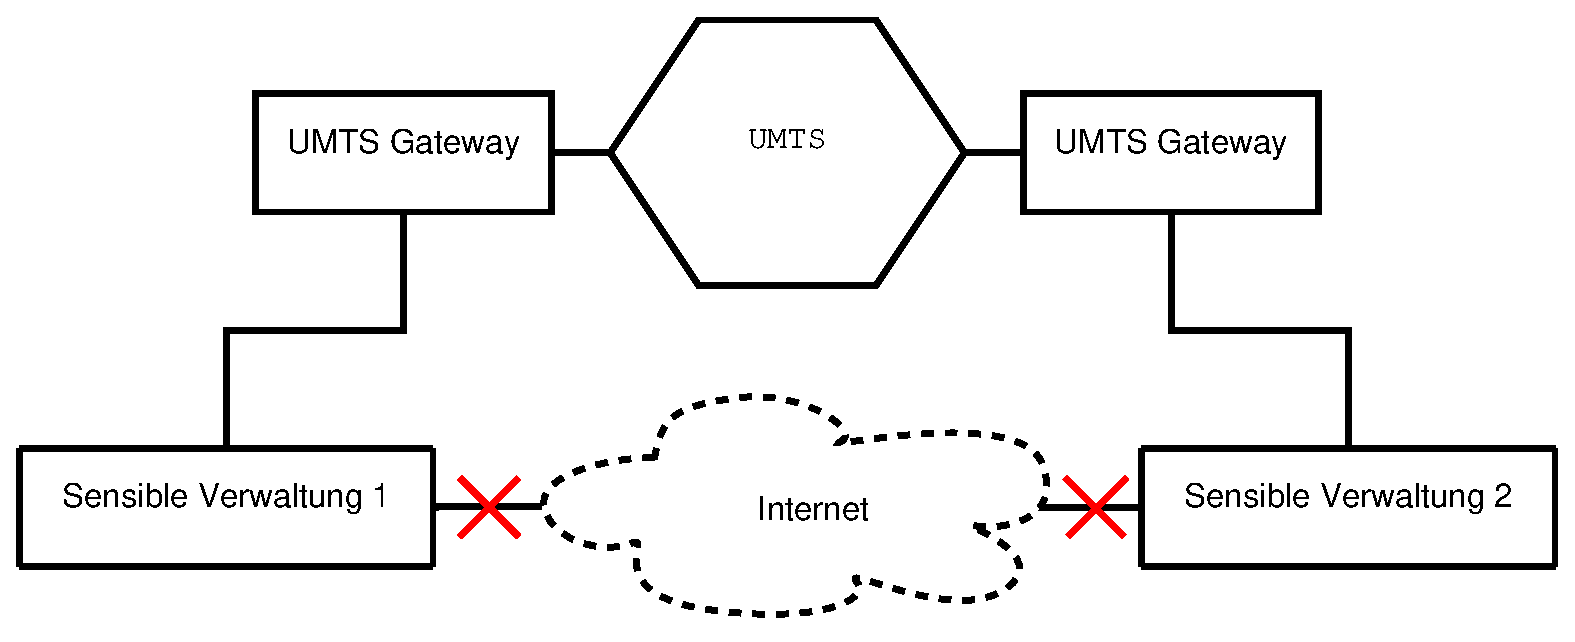
\includegraphics[width=0.8\textwidth]{umtsgateway}
\caption{Alternativweg �ber UMTS}
\label{fig:umtsgateway}
\end{figure}

Auf diesem Wege k�nnten sensible Verwaltungsstellen, beispielsweise �ber UMTS, weiterhin miteinander kommunizieren, ohne den Weg �ber Internetrouter beschreiten zu m�ssen. So w�re ein Datenaustausch dieser Verwaltungen auch zum Zeitpunkt eines gr��eren Ausfalls des Internets m�glich. Diese w�rden dann �ber ein UMTS-Gateway kommunizieren, welches die Schnittstelle zwischen UMTS und dem internen Netzwerk bildet.

Diese Variante ist jedoch f�r gro�e Webseitenbetreiber keine wirkliche Alternative. Dies w�rde bedeuten, dass jeder einzelne Internetprovider ein solches UMTS Gateway einrichtet. Somit w�rde seinen Kunden erm�glicht, eine direkte Verbindung zu einer beliebigen, jedoch festen Webseite, die ebenfalls �ber ein UMTS-Gateway verf�gen muss, aufzubauen. Diese wird dann bei Bedarf mit dem UMTS-Gateway des Providers verbunden und kann dann vom Kunden des Providers abgerufen werden.

Es ist klar zu erkennen, dass das Erreichen von Webseiten vieler verschiedener Anbieter, von jedem Endbenutzer unm�glich zu realisieren ist, da jede Verbindung zu einer Webseite auch das Herstellen einer neuen UMTS-Verbindung nach sich ziehen w�rde. Bei Millionen von Webseiten weltweit und oftmals tausenden Kunden pro Provider w�re der "`Umweg"' �ber UMTS f�r einzelne Webseite praktisch nicht erreichbar.

Aus der Theorie ist erkennbar, dass es ein breites Spektrum an Gefahren gibt, die Netzwerke, also auch Kritische Infrastrukturen, bedrohen. Diese Bedrohungen m�glichst gering zu halten, sowie die Auswirkungen eines Angriffs zu vermindern oder gar zu eliminieren, ist Aufgabe der zuk�nftigen Forschung. Es m�ssen in Zukunft immer wieder Wege gefunden werden, die den Angreifern das Arbeiten zu erschweren oder es ihnen ganz und gar unm�glich zu machen, Infrastrukturen weltweit zu gef�hrden. Es sind schon einige Mechanismen bekannt und in der Anwendung, jedoch lassen sich findige "`B�sewichte"' immer wieder neue Strategien einfallen, die dann zu neuen Bedrohungen werden. Im nun folgenen praktischen Teil wird ein m�glicher Angriff eines Netzwerks und eine geeignete Gegenma�nahme in einem Simulator implementiert, um die theoretisch erl�uterten Probleme zu illustrieren und die daraus gewonnenen Daten zu bewerten.

\chapter{Praktische Implementierung}
\label{cha:praxis}
Im vorhergehenden Kapitel wurden die theoretischen Grundlagen beleuchtet, die f�r den Angriff eines Netzwerkes von Bedeutung sind. Im Folgenden wird exemplarisch ein Angriffsszenario ausgew�hlt. Dieses wird in einem Netzwerksimulator visualisiert und untersucht. Dieser Angriff wird dabei mit einer geeigneten Ma�nahme bek�mpft.

\section{Auswahl eines Szenarios}
Der Grundgedanke bei der Implementierung ist die Sicherstellung eines Nachrichtenaustauschs w�hrend eines Netzwerkangriffs. Hierbei l�sst sich eine Kritische Infrastruktur simulieren, deren Kommunikationssystem unter allen Umst�nden noch funktionieren sollte, wenn ein Angriff gestartet wird. Als Beispiel l�sst sich hier ein Atomkraftwerk anf�hren, dessen Sensoren und Kontrollstationen �ber ein Netzwerk kommunizieren. Deren Kommunikation ist f�r die Aufrechterhaltung der Sicherheit eines Kraftwerks von immenser Bedeutung.

Als weiteres Beispiel sei hier die eMail-Kommunikation zwischen Banken, die beispielsweise auf diesem Weg Informationen �ber das aktuelle B�rsengeschehen austauschen, angef�hrt. Ein Ausfall oder gar Manipulation dieser Kommunikation k�nnte m�glicherweise zu finanziellen Sch�den bei Anlegern aber auch bei der bankinternen Bilanz f�hren.

Die verschiedenen Kommunikationsvarianten k�nnen nun auf den vier verschiedenen Ebenen der Netzwerkstruktur angegriffen werden.
\begin{enumerate}
 \item Physikalische Ebene, z.B. durch Lichtwellen
 \item Netzwerkebene, z.B. IP
 \item Transportebene, z.B. TCP
 \item Applikationsebene, z.B. HTTP
\end{enumerate}
Jede dieser Ebenen ist potentiell angreifbar. Im folgenden werden die einzelnen Ebenen nach m�glichen Gefahrenpunkten hin untersucht, und Varianten erl�utert, die den Nachrichtenaustausch trotz eines Angriffs dieser Ebene noch gew�hrleisten. Die Gew�hrleistung dieses Nachrichtenaustauschs wird im weiteren Verlauf so definiert, dass es bedeutet, dass die Kommunikation, wie sie vor dem Angriff stattgefunden hat, auch w�hrend bzw. nach dem Angriff weiterhin so funktioniert, als h�tte kein Angriff stattgefunden.

Jede Ebene ist von der unter ihr liegenden Ebene abh�ngig. Das hei�t, je weiter unten der Angriff im Ebenenmodell stattfindet, desto gr��er ist die Beeintr�chtigung des gesamten Netzwerks.

\begin{description}
\item[Physikalische Ebene] Ein Angriff auf unterster Ebene ist die wirkungsvollste, wenn auch nicht praktikabelste Variante. Ein solcher Angriff w�re beispielsweise das einfache Kappen eines Kabels oder auch die gewaltsame, physische Zerst�rung eines Routers.

Gegenma�nahmen f�r diese Art von Angriff sind ebenfalls physisch. So sind sensible Rechnersysteme in speziell gesicherten R�umen untergebracht, deren Zutritt nur autorisierten Personen m�glich ist. Kabelstr�nge k�nnen zum einen verzweigt werden um einem \textit{Single-Point-Of-Failure} zu umgehen, zum anderen aber auch in massive Kabelrohre eingebettet werden, um einen physischen Zugang zu erschweren.

\item[Netzwerkebene] Auf dieser Ebene befinden sich die Router. Dortige Angriffe k�nnen entweder direkt auf die Router zielen oder auf Routingprotokolle, mit deren Algorithmen das korrekte Weiterversenden von eingehenden Paketen berechnet wird.

Eine Ma�nahme zur Verhinderung von Angriffen bzw. zur Gew�hrleistung des Routings liegt in der Verschl�sselung von Paketen, im speziellen in der Verschl�sselung von Routinginformationen. Durch eine solche Ma�nahme wird es dem Angreifer erschwert, die enthaltenen Informationen auszulesen oder zu manipulieren.

\item[Transportebene] Ein Angriff auf der Transportebene ist beispielsweise SYN-Flood. Hierbei wird der Verbindungsstatus von TCP ausgenutzt um einen Server zu blockieren.

Eine Gegenma�nahme w�re hierbei ein alternativer Transport �ber UDP, bei dem die Applikationsebene die zus�tzlichen Funktionen von TCP nachbildet. Eine andere M�glichkeit w�re die Beschr�nkung der Anzahl von frei zu vergebenen TCP-Ports. So k�nnte eine Liste erstellt werden, die nur autorisierten Nutzern einen TCP-Port zur Verf�gung stellt.

\item[Applikationsebene] Bei Angriffen auf Applikationsebene geht es im einzelnen um die Serverdienste. So werden immer wieder Sicherheitsl�cken in Serverapplikationen entdeckt, die dem Angreifer erm�glichen sensible Konfigurationen des Servers zu �ndern oder auch diesen zum Absturz zu bringen.

Die bedeutendste Gegenma�nahme ist die regelm��ige Installation von Sicherheitsupdates der Serverssoftware. Diese Updates schlie�en die vorhandenen, bekannten Sicherheitsl�cken. Im Weiteren k�nnte �berlegt werden, die gesamte Serverapplikation redundant auszulegen, und eine zweite Serverapplikation mit Software eines anderen Entwicklerteams zu nehmen. In seltenen F�llen besitzen zwei verschiedenen Serverapplikationen die gleichen Sicherheitsl�cken. So k�nnte beim gezielten Angriff auf die L�cke des einen Servers der andere Server alternativ die Aufgaben des angegriffenen Servers �bernehmen.
\end{description}

\section{Der Simulator}
Die gew�hlte Implementierung eines Angriffs auf ein Netzwerk wurde in einem Netzwerksimulator realisiert. Dieser Simulator ist eine Entwicklung des DAI-Labors\footnote{\url{http://www.dai-labor.de}} der TU-Berlin. Der Simulator dient der Entwicklung und des Testens von neuer Sicherheitssoftware. So k�nnen beispielsweise verschiedene Intrusion-Detection-Systeme (siehe Abschnitt~\ref{sec:ids}) auf ihre Wirksamkeit �berpr�ft werden.

Auf Basis von Eclipse\footnote{\url{http://www.eclipse.org}} als Entwicklungsumgebung, der Programmiersprache Java und JIAC als ein auf Agententechnologien beruhendes Serviceware-Framework wurde der Simulator entwickelt. Eine grafische Benutzeroberfl�che erm�glicht den Aufbau eines simulierten Netzwerkes ohne tiefer gehende Kenntnisse der zugrunde liegenden Architektur der Software. Beispielsweise k�nnen Web-Clients, Web-Server und Router platziert und �ber simulierte Netzwerklinks miteinander verbunden werden. Weitere Ger�te, die bisher in den Simulator eingebunden worden sind: Mail-Server und Proxy-Server.

Bei der Realisierung der Netzwerkverbindungen wurde bewusst auf die Java-Netzwerk\-sockets verzichtet. Alternativ wurden eigene Sockets programmiert, die auf der TCP/IP-Archi\-tektur aufbauen. So gibt es einen IP-Layer, der f�r das Erstellen von IP-Paketen sowie deren Fragmentierung zust�ndig ist. Es gibt dar�ber hinaus einen Network-Layer, der das Routing steuert und einen Transport-Layer, indem die Funktionalit�t von TCP und UDP abgebildet wird. Jedes Ger�t im Netzwerk enth�lt demnach ein System aus mehreren Ebenen, die jede f�r sich spezielle Aufgaben erf�llen. Au�erdem existiert auf den Endger�ten, also Servern und Clients, noch eine Applikationsebene, welche die Server- bzw. Client-Applikationen enth�lt.

\subsection{Relevante Ger�te}
Die f�r die Implementierung des Angriffsszenarios relevanten Ger�te sind Web-Clients, Web-Server und Router.
\begin{description}
\item[Web-Client] Der Web-Client ist in der Lage Webseiten von allen Web-Servern, die im gesamten Netzwerk vorhanden sind, anzufordern. Dazu wird auf der Applika\-tionsebene des Clients ein HTTP-Request generiert und dort an die unteren Netzwerkebenen weitergegeben. Kommt auf dieses HTTP-Request ein HTTP-Response, also eine Antwort vom Web-Server, zur�ck, so wird diese im Browserfenster angezeigt.

\item[Web-Server] Der Web-Server wartet auf HTTP-Requests von Web-Clients. Erh�lt er ein solches Request, so wird ein Server-Thread gestartet, der dann wiederum die Antwort an den anfragenden Client zur�cksendet. Dies geschieht konform zur Spezifikation des HTTP-Protokolls.

\item[Router] Die Router sind f�r die Verteilung der IP-Pakete im Netzwerk zust�ndig. F�r das Erstellen seiner Routinginformationen nutzt der Router standardm��ig OSPF (\textit{Open Shortest Path First}), ein Link-State Routing Protokoll. Wahlweise l�sst sich hier auch ISIS (\textit{Intermediate System to Intermediate System Protocol}) als Routingprotokoll einstellen.
\end{description}

Der einfache Aufbau eines Netzwerks, bestehend aus mehreren Web-Servern, Web-Cients und Routern, k�nnte dann so aussehen, wie z.B. in Abbildung~\ref{fig:beispielaufbau}.
\begin{figure}[htb]
\centering
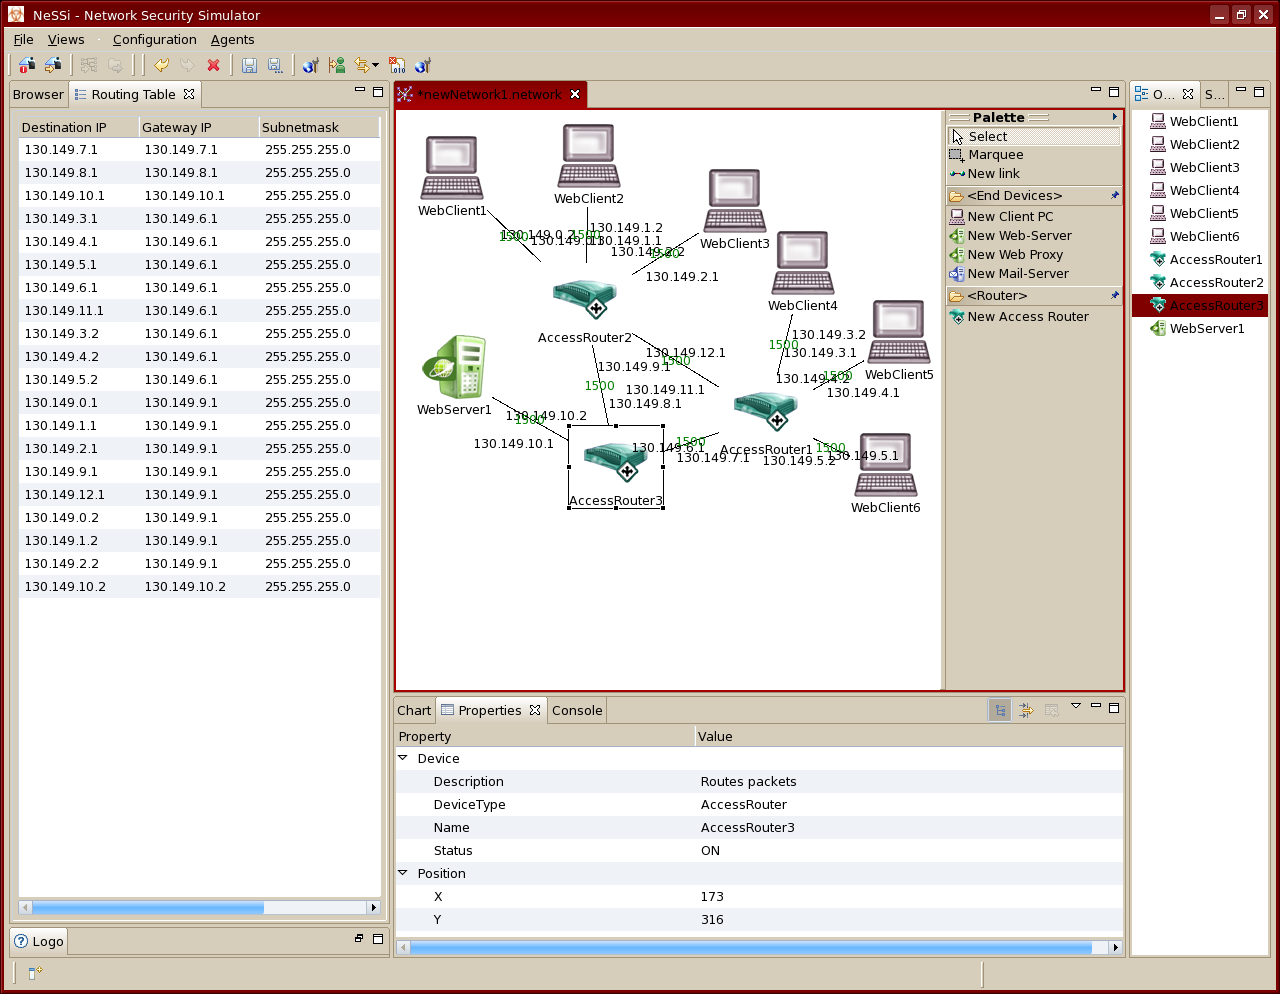
\includegraphics[width=0.8\textwidth]{beispielaufbau}
\caption{Beispielhafter Aufbau eines kleinen Netzwerks in NeSSi}
\label{fig:beispielaufbau}
\end{figure}

Dies ist die Ausgangsimplemetierung des Netzwerksimulators NeSSi. Sie wird nun anhand eines ausgew�hlten, beispielhaften Angriffsszenarios erweitert. Dieser Angriff soll folgend mit einer Gegenma�nahme abgeschw�cht werden, so dass ein Nachrichtenaustausch weiterhin m�glich ist. Diese Ma�nahme wird ebenfalls in den Simulator integriert und dort getestet.

\section{Implementierung}
Wie in Abschnitt~\ref{sec:trojaner} schon erw�hnt wurde, werden DDoS-Angriffe in der Regel �ber einen IRC gestartet. Dazu sind eine gro�e Anzahl, beispielsweise �ber Trojaner infizierter Rechner �ber ein IRC-Netzwerk miteinander verbunden und k�nnen so kommunizieren. Der Angreifer hat daf�r gesorgt, dass er nun viele Rechner weltweit ansteuern und ihnen Befehle erteilen kann. Sie wurden zu Bots. Es kann Befehle absetzen, die z.B. einen SYN-Flood auf ein bestimmtes Ziel veranlassen. Alle verbundenen Bots erhalten diesen Befehl und werden das, vom Angreifer gew�nschten Ziel, mit SYN-Paketen "`bombardieren"'. Dieses Vorsehen f�hrt dazu, dass viele TCP-Verbindungen ge�ffnet werden. Die Verbindungen sind jedoch nicht komplett ge�ffnet, da das Antwortpaket des Angreifenden ausbleibt (3-Wege-Handshake: siehe Abschnitt~\ref{sec:synflood}). Da das Betriebssystem nur begrenzt halboffene Verbindungen bereit stellt, ist es ab einem gewissen Zeitpunkt nicht mehr m�glich, neue TCP-Verbindungen zu �ffnen. Dies schlie�t auch die Versuche von Benutzern ein, die nicht Teil des Angriffs sind. 

Hier muss die Gegenma�nahme ansetzen. W�hrend eines solchen DDoS-Angriffs, eines SYN-Floods, sollen trotzdem noch neue TCP-Verbindungen m�glich sein. Hierzu muss f�r legitime neue Verbindungen eine Reserve zur�ckgehalten werden. Aus dieser Reserve werden nur dann neue Verbindungen entnommen, wenn die Anfrage von einer autorisierten Stelle kommt. Die IP-Adressen autorisierter Clients werden in einer \textit{Whitelist} gespeichert, die sowohl statische als auch dynamische Elemente enth�lt. Ein bestimmter Anteil der maximal m�glichen Anzahl an halboffenen Verbindungen wird f�r diese Whitelist reserviert.

\subsection{IRC-Szenario}
F�r die Realisierung eines Angriffs mittels eines IRC-Netzwerks, sind weitere Ger�te im Simulator zu entwickeln. Zum einen wird ein Angreifer ben�tigt, der die einzelnen Bots mit Hilfe des IRC-Protokolls steuert und ihnen den Befehl zum SYN-Flood eines ausgew�hlten Ziels erteilt. Dieses Ziel k�nnte beispielsweise ein Web-Server sein.

Zum anderen wird f�r die Kommunikation der Bots und des Angreifers ein IRC-Server ben�tigt. Dieser IRC-Server ist als vermittelnde Einheit zwischen den Bots und dem Angreifer zu sehen. Alle Bots sind auf diesem IRC-Server eingew�hlt, und sind Teilnehmer desselben IRC-Kanals auf diesem Server.

Neben diesen neuen Endger�ten ist auch noch die Modifizierung der Web-Clients n�tig. Damit diese Clients nicht nur in der Lage sind Webseiten von diversen Web-Servern abzurufen sondern auch SYN-Floods zu t�tigen, ist daf�r zu sorgen, dass sie als Bots in einem Bot-Netzwerk teilnehmen k�nnen. Diese Bots k�nnen sich auf einem beliebigen IRC-Server einw�hlen und dort in einem definierten IRC-Kanal auf Anweisungen warten. 

\subsubsection{IRC-Server}
Zur Integration des IRC-Servers wurde eine bereits bestehende GPL-lizenzierte Implementierung namens \textit{Sonata IRC Network}\footnote{\url{http://sourceforge.net/projects/sonata/}} genutzt. Es wurde ein neues Ger�t erstellt, auf dem im Basiszustand ein Thread l�uft, der diesen IRC-D�mon enth�lt. Als IRC-D�mon wird im weiteren Verlauf die verwendete Software des IRC-Servers bezeichnet. Die Implementierung dieses IRC-D�mons musste an die Socketimplementierung von NeSSi angepasst werden.

In der Version mit Java-Sockets wird im IRC-D�mon der Server-Socket erstellt. Dieser wartet dann auch eingehende Verbindungen. Gehen Anfragen auf neue TCP-Verbindun\-gen ein, so wird ein Client-Socket erstellt, der dann wiederum einem neu erstellten Client-Thread �bergeben wird. Dieser neu erstellte Thread kommuniziert �ber den �bergeben Socket mit dem IRC-Client.

Mit der Socket-Implementierung von NeSSi muss dies im geringen Umfang ummodelliert werden. Hier wird bereits in der IRC-Server-Applikation, die den IRC-D�mon als Thread enth�lt der Server-Socket kreiert. Dieser wird dem IRC-D�mon �bergeben. Eingehende Verbindungsanfragen auf dem erzeugten Server-Socket werden in der Transportebene behandelt. Dort wird ein Client-Socket erstellt, der an die Applikationsebene des IRC-Servers weitergegeben wird. Dort wird der erhaltenen Client-Socket wiederum an den IRC-D�mon �bergeben, der dann intern einen neuen Client-Thread mit diesem erhaltenen Socket erstellt.

\subsubsection{Bots}
Der Web-Client in der Ausgangsversion enth�lt Applikationen zum Browsen und zur Versendung von UDP-Paketen. Um nun die Kommunikation mit einem IRC-Server m�glich zu machen muss auf dem Web-Client eine weitere Applikation laufen, die die Verbindung zum IRC-Server steuert. Diese Applikation hei�t Bot-Applikation. Auch f�r diese Applikation wurde eine bereits existierende Implementierung eines IRC-Clients mit dem Namen PircBot\footnote{\url{http://www.jibble.org/pircbot.php}} benutzt. Die Bot-Applikation des Web-Clients besitzt einen Thread, der diesen PircBot enth�lt.

Auch die Implementierung des PircBot musste f�r die eigene Socket-Implementierung von NeSSi umgestaltet werden. Sobald die Verbindung zu einem IRC-Server aufgebaut werden soll, wird auf der Transportebene des Web-Clients ein Client-Socket erzeugt. Dieser Socket kann von der Bot-Applikation benutzt werden. Folgend wird dieser erzeugte Socket an den PircBot weitergegeben. Innerhalb des PircBot ist die Erstellung eines Sockets demnach nicht n�tig. Der erhaltene Socket kann somit zur Einwahl auf dem IRC-Server und zur weiteren Kommunikation mit diesem genutzt werden.

Um von der grafischen Benutzerschnittstelle in der Bot-Applikation eines Web-Clients die Einwahl auf einem vorhandenen IRC-Server zu erreichen, wird ein Event generiert, welches Daten zur IP-Adresse des IRC-Servers und dem IRC-Kanal enth�lt. Diese Daten wurden zuvor �ber einen Dialog ermittelt. Der generierte Event l�st in der Bot-Applikation des Web-Clients die Ausf�hrung einer bestimmten Methode aus. Diese Methode erzeugt dann den Thread, der mittels des PircBot und der �bermittelten Daten eine TCP-Verbindung mit dem IRC-Server herstellt, und auf dem IRC-Server dem gew�nschten IRC-Kanal beitritt.

Nach der erfolgreichen Einwahl ist der Web-Client nun ein Bot, der auf eingehende Textnachrichten wartet. Speziell codierte Textnachrichten, die vom Angreifer in dem IRC-Kanal gesendet werden, l�sen in der Bot-Applikation bestimmte Reaktionen aus.

\subsubsection{Angreifer}
Der Angreifer enth�lt, genau wie der Web-Client, eine Bot-Applikation. Auch hier wird, ausgehend von der grafischen Oberfl�che, ein Event generiert, welches die Bot-Applikation dazu veranlasst, einen Thread mit enthaltenem PircBot zu starten. Hier wird �ber einen Dialog der IRC-Server und IRC-Kanal gew�hlt. Zus�tzlich wird ein Befehl erwartet, der allen Bots, die auf gew�hlten IRC-Kanal des gegebenen IRC-Servers auf Nachrichten warten, gesendet wird. F�r die Ausf�hrung eines SYN-Floods wird folgende Syntax als Textnachricht versendet:
\begin{quotation}
\texttt{synflood <ip1> <ip2> <count>}
\end{quotation}
\texttt{ip1} ist hierbei die gespoofte Absenderadresse des SYN-Pakets, \texttt{ip2} die Zieladresse. \texttt{count} bezeichnet die Anzahl der zu sendenden SYN-Pakete pro Bot. Wird nun \texttt{synflood 130.149.5.2 130.149.11.2 1000} an Kanal X des IRC-Servers Y gesendet, so werden alle Bots, die auf Kanal X des IRC-Servers Y horchen, einen SYN-Flood auf den Rechner mit der IP \texttt{130.149.11.2} starten und sich als \texttt{130.149.5.2} ausgeben. Die Flutung besteht aus $1000$ SYN-Paketen.

Ein solches SYN-Flood k�nnte nun auf einen Web-Server zielen. Der Aufbau eines einfachen Netzwerks ist in Abbildung~\ref{fig:ircszenario} zu sehen. Teilnehmer des Netzwerks sind IRC-Server, Angreifer (Attacker), Bots (Web-Clients) und ein anzugreifender Web-Server.
\begin{figure}[htb]
\centering
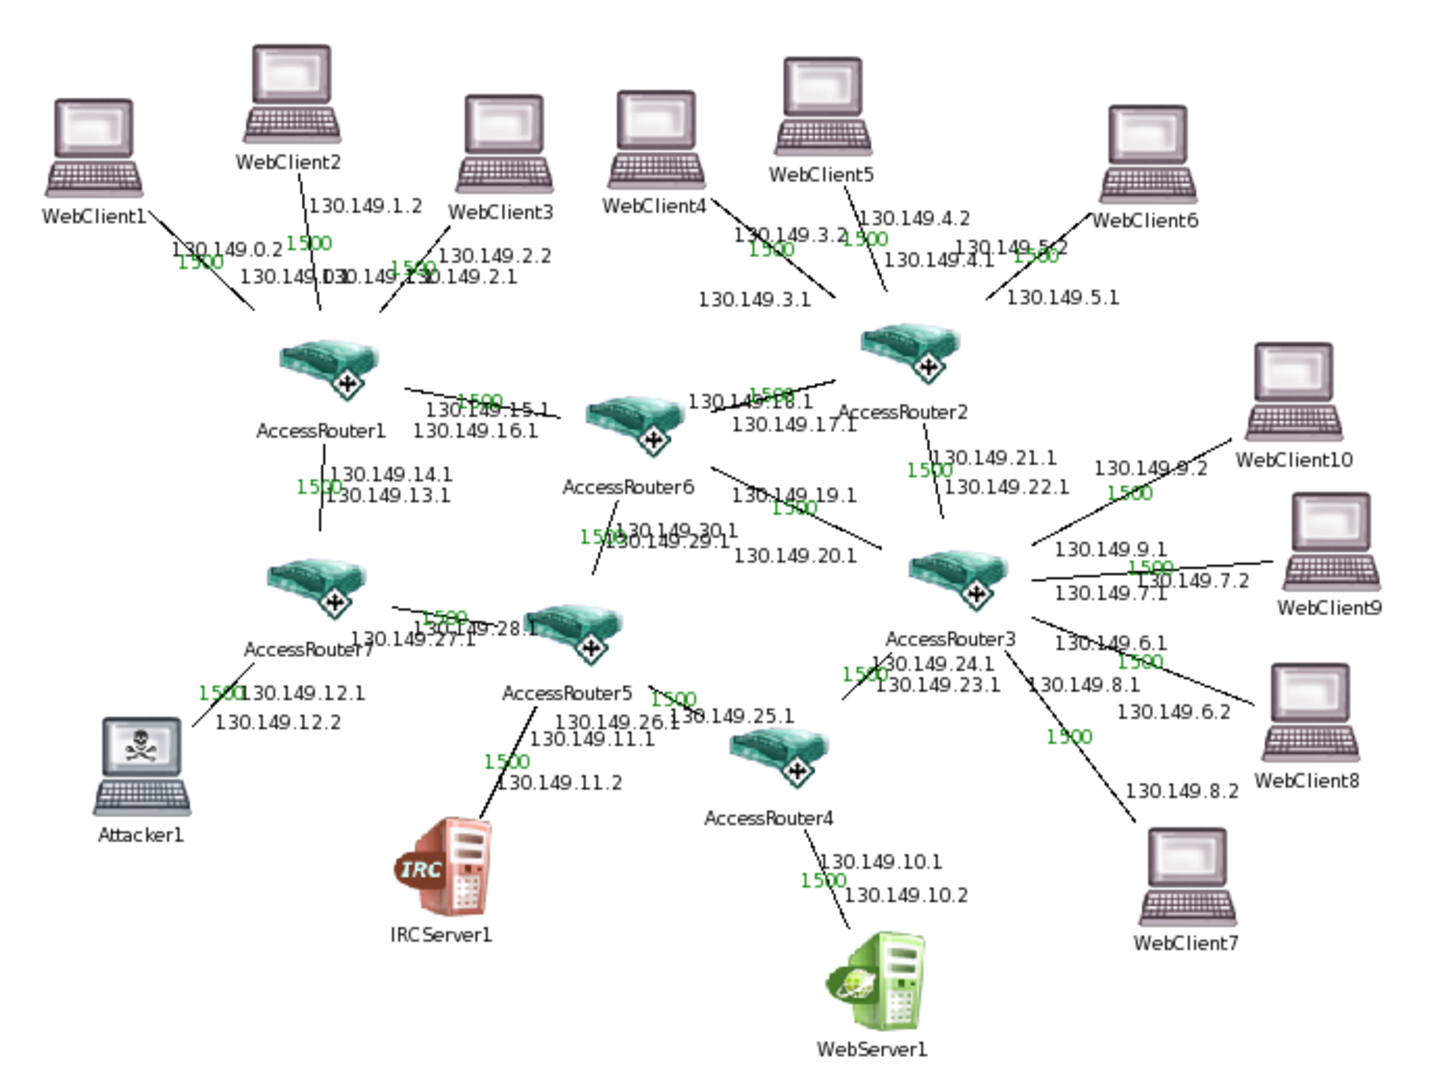
\includegraphics[width=0.8\textwidth]{ircszenario}
\caption{Aufbau eines Gesamtsystems im Angriffsszenario}
\label{fig:ircszenario}
\end{figure}

\subsection{Halboffene Verbindungen in TCP}
Da in der bestehenden Implementierung von NeSSi die Limitierung von halboffenen TCP-Verbindungen noch nicht eingebaut ist, musste diese zun�chst verwirklicht werden. Zu diesem Zweck wurde eine Klasse \textit{HalfOpenedConnections} entwickelt, welche diese halboffenen Verbindungen verwaltet. Sie enth�lt eine Liste von (Socket,Zeit)-Paaren, die mit Hilfe der enthaltenen Methoden aktualisiert werden. Jedes Element der Liste besteht demnach aus einem Socket und einem Zeitstempel, der f�r die sp�tere Aktualisierung der Liste notwendig ist.

Bei jeder eingehenden Anfrage einer TCP-Verbindung, also dem Erhalt eines SYN-Pakets wird der erzeugte Client-Socket in die Liste der halboffenen Verbindungen eingef�gt. Beim Einf�gen wird als Zeitstempel die aktuelle Zeit benutzt.

Beim Erhalt eines ACK-Pakets, also der Best�tigung der Verbindung �ndert sich der Status der TCP-Verbindung von \textit{halboffen} nach \textit{offen}. Somit kann der Socket, dem dieses TCP-Verbindung zugeordnet wird aus der Liste der halboffenen Verbindungen entfernt werden.

Neben der Entfernung nach erfolgreichem Verbindungsaufbau gibt es noch die M�glichkeit eines \textit{timeout}. Sollte nach einer definierten Zeit kein ACK-Paket zur Best�tigung der TCP-Verbindung eintreffen, so wird der Socket, dessen "`Zeit abgelaufen ist"', zur Schonung von Ressourcen aus der Liste genommen. Die �berpr�fung solcher \textit{timeouts} geschieht direkt nach dem Eintreffen eines neuen SYN-Pakets. Dabei wird f�r alle Elemente in der Liste �berpr�ft, ob die aktuelle Zeit vor oder nach der Zeit liegt, die sich ergibt, wenn Zeitstempel und timeout-Zeit addiert werden. Liegt die errechnete Zeit nach der aktuellen Zeit, so liegt ein timeout vor und das zugeh�rige Element wird aus der Liste gel�scht.

\subsection{Whitelist-Prinzip}
Mit der Implementierung der begrenzten Liste von halboffenen Verbindungen ist nun f�r die Angreifer die M�glichkeit gegeben, diese Begrenzung zu missbrauchen. Da nun nur begrenzt halboffene Verbindungen m�glich sind, erreicht der Angreifer mit einem SYN-Flood den Effekt, dass legitime Anfragen bei voller Liste von halboffenen Verbindungen ignoriert werden.

Hier setzt die Whitelist an. Beispielsweise die H�lfte der begrenzten Anzahl an halboffenen Verbindungen wird nun nur noch f�r Anfragen benutzt, deren Quell-IP-Adresse in der Whitelist enthalten sind. Diese Whitelist enth�lt zwei verschiedene Listen. Eine statische Liste, welche IP-Adressen enth�lt, die f�r unbegrenzte Zeit priorisiert werden sollen. Zum zweiten gibt es eine dynamische Liste, deren Eintr�ge laufend ge�ndert werden. So wird eine IP-Adresse in diese dynamische Liste eingef�gt, wenn sie die TCP-Verbindung regul�r, also mit einem FIN-Paket, beendet. So wird erreicht, dass Angreifer, die nur SYN-Pakete senden, in diese Liste aufgenommen werden. 

Wie auch bei der Liste der halboffenen Verbindungen bekommt jede IP-Adresse, die in die dynamische Liste eingef�gt wird, einen Zeitstempel zugeordnet. Jeder Eintrag darf nur f�r eine fest definierte Zeit in der dynamischen Liste gef�hrt werden. Sie ist nach dem gleichen Prinzip timeout-gesteuert wie die Liste der halboffenen Verbindungen. Somit ist gew�hrleistet, dass die dynamische Liste nicht zu gro� wird und irgendwann so viele IP-Adressen enth�lt, dass die gespooften Absender-IP-Adressen der SYN-Floods in zu gro�er Anzahl in der Liste vorhanden sind, und die Whitelist ihre Wirkung verliert.

Um diese Implementierung zu testen, wurden verschiedene Szenarien erstellt.

\section{Test}
Um die Funktionalit�t und Wirksamkeit des Whitelist-Ansatzes zu testen, wurde ein Netzwerkaufbau (Abbildung~\ref{fig:testaufbau}) konstruiert.
\begin{figure}[htb]
\centering
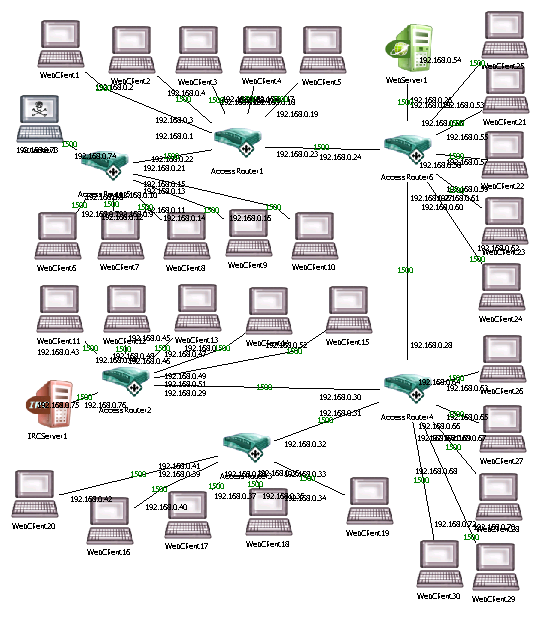
\includegraphics[width=0.7\textwidth]{testaufbau}
\caption{Testaufbau}
\label{fig:testaufbau}
\end{figure}
In diesem Netzwerk existieren 30 Web-Clients, ein Web-Server, ein IRC-Server und eine Attacker. In drei verschiedene Szenarien wurden Daten gesammelt.

\subsection{Szenario 1}
Im ersten Szenario hat jeder der 20 Web-Clients auf der linken Seite alle $0,5$ Sekunden einen Browse-Versuch unternommen. Jeder der Web-Clients kann vier Browse-Vorg�nge gleichzeitig durchf�hren. Die Liste der halboffenen TCP-Verbindungen auf dem Web-Server hat eine L�nge von $100$.

\subsection{Szenario 2}
Im zweiten Szenario t�tigte wiederum jeder der 20 Web-Clients Browse-Versuche. Hierbei wurde nun ein DDoS Angriff auf den Web-Server unternommen. Die 10 Web-Clients, die sich rechts befinden, registrierten sich dazu beim IRC-Server. Der Attacker registrierte sich ebenfalls beim IRC-Server und gab den Befehl des SYN-Flood auf den Web-Server. Alle $0,2$ Sekunden wurde von jedem Web-Client ein SYN-Paket an den Web-Server gesendet.

\subsection{Szenario 3}
Auch im dritten Szenario t�tigte jeder der 20 Web-Clients Browse-Versuche. Auch hier wurde ein DDoS Angriff auf den Web-Server unternommen. Weiterhin wurde auf dem Web-Server das Whitelist-Prinzip aktiviert. Jede erfolgreicher Verbindungsaufbau f�hrte dazu, dass der, dieser Verbindung zugeordnete Client, in die Whitelist aufgenommen wurde.

\subsection{Auswertung}
In jedem Szenario wurden Daten in einer Datei gespeichert. Sowohl die versuchten, als auch die erfolgreich aufgebauten Verbindungen wurden registriert. Die Daten wurden in ein Diagramm, wie in Abbildung~\ref{fig:diagramm}, exportiert. Der Web-Server hat eine Beschr�nkung in der Anzahl der halboffenen Verbindungen. Es sind im Zustand ohne Whitelist-Prinzip $100$ halboffene Verbindungen m�glich. Jede weitere Verbindungsanfrage wird verworfen.
\begin{figure}[htb]
\centering
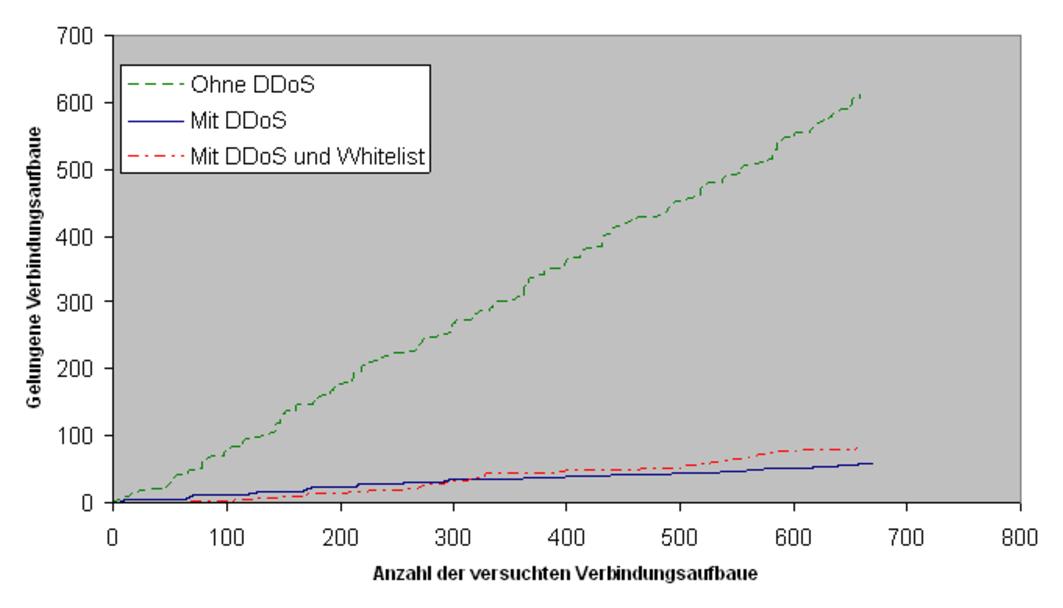
\includegraphics[width=0.9\textwidth]{diagramm}
\caption{Auswertungsdiagramm}
\label{fig:diagramm}
\end{figure}

Es ist zu erkennen, dass die Kurve des ersten Szenarios ("`Ohne DDoS"') kontinuierlich und ann�hernd linear steigt. Dies war aufgrund des Testaufbaus auch so zu erwarten. Da alle 20 Web-Clients insgesamt maximal 80 Browse-Anfragen stellen k�nnen, wurde die maximale Anzahl an halboffenen Verbindungen des Web-Servers nicht erreicht. Daher wird jede Anfrage akzeptiert. Es ist anzumerken, dass die Kurve aufgrund eines geringeren Datenvolumens k�nstlich verl�ngert wurde. Dies dient der Vergleichbarkeit der Kurven. Es ist m�glich, da die Kurve linear verl�uft.

Beim zweiten Szenario ("`Mit DDoS"') werden wesentlich weniger Verbindungen zugelassen. Dies resultiert aus dem SYN-Flood. Dieser bewirkt eine st�ndige �berf�llung der Liste an halboffenen Verbindungen im Web-Server. Nach einem Timeout von $30$ Sekunden wird jede Verbindungsanfrage verworfen. Es besteht daher immer wieder die M�glichkeit, dass nicht jede legitime Verbindungsanfrage verworfen wird. Legitim sind hierbei die Browse-Anfragen der 20 Web-Clients. Die Anzahl der gelungenen Verbindungsaufbaue f�llt mit $10\%$ jedoch sehr gering aus.

Die Kurve des dritten Szenarios ("`Mit DDoS und Whitelist"') verl�uft �hnlich wie die des zweiten Szenarios. Es ist jedoch zu sehen, dass ab einer Anzahl von etwa $300$ Anfragen die Kurve eine h�here Steigung aufweist. Dies ist dadurch zu erkl�ren, dass die aktivierte Whitelist den Aufbau von legitimen neuen Verbindungen erleichtert. Der Web-Server reserviert 50 Pl�tze auf der Liste der halboffenen Verbindungen f�r Mitglieder der Whitelist. Diese Pl�tze sind vom SYN-Flood nicht betroffen. Mit fortlaufender Zeit werden immer mehr legitime Web-Clients Mitglieder der Whitelist. Somit steigt die Wahrscheinlichkeit eines erfolgreichen Verbindungsaufbaus.

Insgesamt ist zu erkennen, dass der Whitelist-Ansatz eine L�sung anbietet. Die Wirkung ist jedoch gering. Weitere Bewertungen und Ausblicke werden in dem folgenden Fazit er�rtert.

\chapter{Fazit}
\label{cha:fazit}
Aus dem Diagramm (Abbildung~\ref{fig:diagramm}) ist die Wirksamkeit des Whitelist-Ansatzes zu erkennen. Mit steigender Versuchsdauer erh�ht sich die Wahrscheinlichkeit eines erfolgreichen Verbindungsaufbaus, deren Wirkung jedoch nur sehr gering ist. Es ist zu erwarten, dass in einem l�nger andauernden Szenario, die Kurve "`Mit DDoS und Whitelist"' noch weiter an Steigung zunimmt. Dies liegt in der Aufnahme von weiteren Web-Clients in die Whitelist begr�ndet.

W�hrend eines stattfindenden SYN-Flood ist die Aufnahme in die Whitelist nur schwer m�glich. Ein Timeout verkleinert die Liste der halboffenen Verbindungen um jeweils ein Element. Nur in diesem Fall besteht M�glichkeit, dass eine Anfrage nicht verworfen wird. Da neben den Anfragen der Web-Clients aber weiterhin noch SYN-Pakete von Bots gesendet werden, ist die Wahrscheinlichkeit sehr gering, dass der Anfrage des Web-Clients genau dieser frei gewordene Platz zugeteilt wird. Nur wenn das SYN-Paket des legitimen Web-Clients nicht verworfen wird, besteht die M�glichkeit, dass die Verbindung zustande kommt. Einzig in diesem Fall wird der Web-Client in die Whitelist aufgenommen.

In diesem Punkt zeigt das Whitelist-Prinzip einen Schwachpunkt. Der Angreifer k�nnte beispielsweise die Methodik der Aufnahme in die dynamische Whitelist erraten oder durch Probieren heraus finden.

Bei dem hier implementierten Ansatz erfolgt die Aufnahme nach dem Senden eines ACK-Pakets. Die Bots des Angreifers k�nnten ein solches Paket aber auch senden. Damit w�rden sie in die Whitelist aufgenommen. Dies h�tte die Unwirksamkeit der Whitelist zur Folge.

Diese Whitelist-Methode ist nur eine von vielen Methoden zur Abwehr von Angriffen bzw. zur Begrenzung von Sch�den durch Angriffe. Mit Hilfe von NeSSi k�nnten sich weitere Strategien entwickeln lassen. Das Einbinden des IRC-Protokolls als Kommunikationsmedium f�r Angreifer und Bots hat dem Simulator zus�tzliche Flexibilit�t verliehen. Auf dieser Grundlage best�nde die M�glichkeit, weitere Gegenma�nahmen zur DDoS-Abwehr zu entwickeln und weitere Angriffsszenarien zu implementieren. Die implementierte Kommunikation �ber IRC er�ffnet Perspektiven zuk�nftiger Forschungsanstrengungen.


% Setze Numerierung wieder auf r�misch zur�ck und setzte von oben fort
% Wert ist demnach der von 'roemisch'
\newpage
\pagenumbering{Roman}
\setcounter{page}{\value{roemisch}}

% Literaturverzeichnis
\bibliography{literatur/bib}

% Appendix, falls vorhanden
%\appendix
%\chapter{Anhang Eins}

\chapter*{Erkl�rung der Urheberschaft}
\label{sec:urheber}

Ich erkl�re hiermit an Eides statt, dass ich die vorliegende Arbeit
ohne Hilfe Dritter und ohne Benutzung anderer als der angegebenen
Hilfsmittel angefertigt habe; die aus fremden Quellen direkt oder
indirekt �bernommenen Gedanken sind als solche kenntlich gemacht. Die
Arbeit wurde bisher in gleicher oder �hnlicher Form in keiner anderen
Pr�fungsbeh�rde vorgelegt und auch noch nicht ver�ffentlicht.


\vspace{4cm}

\hspace{2cm} Ort, Datum \hfill Unterschrift \hspace{2cm}


\end{document}
